\chapter{Aspectos teóricos y prácticos de OCT} \label{chapter:aspectos_teo_y_pract_oct}
%\section{Introducción}

En este capítulo se abarcarán los conceptos básicos relacionados con OCT, mostrando su desarrollo desde el fundamento de la interferometría con luz blanca hasta finalizar con el sistema de medición que se emplea en OCT. La última parte del capítulo está destinada a los resultados obtenidos con el montaje de prueba que se realizó en el laboratorio y en donde se efectuaron pruebas para dos muestra. Este capítulo se encuentra dividido en cuatro secciones: la Sección~\ref{sec:estado_del_arte} muestra el estado del arte de OCT, pero desde un punto de vista del desarrollo científico que ha tenido; la Sección~\ref{sec:marco_teorico} presenta la teoría que hay detrás del desarrollo mencionado anteriormente; la Sección~\ref{sec:param_important} relaciona algunos parámetros importes que se deben considerar en OCT, y la Sección~\ref{sec:impementacion} expone el sistema óptico implementado en el laboratorio del Grupo de Óptica Aplicada.

\section{Estado del arte de OCT}
\label{sec:estado_del_arte}

%En OCT, la luz retrodispersada se mide empleando interferometría de baja coherencia, también conocida como interferometría con luz blanca, en donde se captura el patrón de interferencia que es producido por un haz de referencia y un haz objeto empleando una fuente con un ancho espectral grande \cite{Tomlins, Fercher}. El haz de referencia es aquel que proviene de la fuente y viaja de manera directa hasta el detector, mientras que el haz objeto es aquella porción de la luz que luego de ser retroreflejada por la muestra, viaja en dirección del detector. Como la fuente tiene un ancho espectral que abarca varias longitudes de onda, la interferencia entre el haz objeto y referencia solo se produce en una región donde la diferencia de camino entre ambos haces se encuentre dentro de la longitud de coherencia \cite{Drexler2015}. Aprovechando este concepto, OCT realiza las medidas interferométricas en profundidad mediante el desplazamiento del haz referencia, produciendo que la interferencia se dé unicamente en la región contenida dentro de la longitud de coherencia. A esa medida de interferencia contra profundidad, se le conoce como escaneo axial, escaneo tipo A (A-scan) o línea tipo A (A-line) \cite{Drexler2015}. Si se desplaza de manera transversal en una única dirección tanto el haz objeto como referencia y luego se realizan múltiples escaneos tipo A, la imagen bidimensional obtenida corresponde a la sección transversal del objeto, a este tipo de escaneo bidimensional se le conoce como escaneo tipo B (B-scan). Finalmente, si se toman múltiples escaneos tipo B de forma perpendicular a los desplazamientos, se obtendrá una imagen tridimensional de la muestra, conociendo la magnitud de los desplazamientos realizados en cada una de las direcciones, puede entonces reconstruirse el volumen \cite{Bouma2002}.

%OCT es una técnica de imagen médica, que se basa en la medición del ``eco'' que se produce cuando la luz llega hasta un tejido. El eco corresponde a aquella porción de luz que luego de llegar al tejido y ser esparcido, se propaga de regreso hasta el sistema óptico. La luz esparcida se mide empleando interferometría de baja coherencia, también conocida como interferometría con luz blanca, en donde se captura el patrón de interferencia que es producido por un haz de referencia y un haz objeto empleando una fuente con un ancho espectral grande \cite{Tomlins, Fercher}. El haz de referencia es aquel que proviene de la fuente y viaja de manera directa hasta el detector, mientras que el haz objeto es aquella porción de la luz que luego de ser esparcida por la muestra, viaja en dirección del detector. Como la fuente tiene un ancho espectral que abarca varias longitudes de onda, la interferencia entre el haz objeto y referencia solo se produce en una región donde la diferencia de camino entre ambos haces se encuentre dentro de la longitud de coherencia \cite{Drexler2015}. Aprovechando este concepto, OCT realiza las medidas interferométricas en profundidad mediante el desplazamiento del haz referencia, produciendo que la interferencia se dé unicamente en la región contenida dentro de la longitud de coherencia. A esa medida de interferencia contra profundidad, se le conoce como escaneo axial, escaneo tipo A (A-scan) o línea tipo A (A-line) \cite{Drexler2015}. Si se desplaza de manera transversal en una única dirección tanto el haz objeto como referencia y luego se realizan múltiples escaneos tipo A, la imagen bidimensional obtenida corresponde a la sección transversal del objeto, a este tipo de escaneo bidimensional se le conoce como escaneo tipo B (B-scan). Finalmente, si se toman múltiples escaneos tipo B de forma perpendicular a los desplazamientos, se obtendrá una imagen tridimensional de la muestra, conociendo la magnitud de los desplazamientos realizados en cada una de las direcciones, puede entonces reconstruirse el volumen \cite{Bouma2002}.

%El surgimiento de OCT se encuentra relacionado con el concepto de medir la magnitud y el tiempo que tarda el ``eco'' en producirse cuando la onda llega hasta el tejido. Es por ello, que el concepto de OCT tuvo su surgimiento en la óptica de femtosegundos, en este sentido, hacia 1971 Michael Duguay propuso emplear obturador de efecto Kerr para obtener fotografías instantáneas de la propagación de la luz. Aunque la velocidad con la que desplaza la luz en el vacío es de $~3\times10^8 m/s$, el obturador de efector Kerr puede alcanzar resoluciones de picosegundos, mediante la inducción de birrefringencia con un láser. Esta tecnología llegó a tener resoluciones axiales (en profundidad) de hasta $15\mu m$, alcanzado una sensibilidad de hasta $-70dB$, o una capacidad de medir un reflector que refleje $10^{-7}$ veces la energía de la onda incidente. Esta tecnología estaría en la medición de tejidos hasta finales de la década de los 80, cuando se realizaran las primeras aplicaciones biológicas de la interferometría de baja coherencia o interferometría de luz blanca. Esos primeros estudios fueron realizados para medir la profundidad del ojo, y servirían como base para el empleo de interferometría de baja coherencia en especímenes biológicos. 

El surgimiento de OCT se encuentra relacionado con el concepto de medir el ``eco'' que se produce cuando la luz interactúa con tejidos, de manera similar a como se hace en ultrasonido. Es por ello, que el concepto de OCT tuvo su origen en la óptica de femtosegundos, liderada por Michael Duguay en la década de los 70 \cite{Duguay1971}. Las primeras mediciones biomédicas con óptica de femtosegundos, fueron realizadas a través del efecto Kerr inducido en un láser, cuya función era controlar un obturador a altas velocidades (del orden de los picosegundos), de forma que el eco de un pulso corto de luz podía ser capturado. Esta tecnología llegó a tener resoluciones axiales de hasta $15\mu m$, alcanzado una sensibilidad de hasta $-70dB$, o una capacidad de medir $10^{-7}$ veces la intensidad de la onda incidente. Este sistema sería empleado en la medición de tejidos hasta finales de la década de los 80, cuando se realizaran las primeras aplicaciones biológicas de la interferometría de baja coherencia o interferometría de luz blanca \cite{Fercher1988}. 

Mediante interferometría con luz blanca, el eco se mide con la captura el patrón de interferencia que es producido por un haz de referencia y un haz objeto empleando una fuente con un ancho espectral grande o banda ancha, definida en el orden de los $10nm$ \cite{Tomlins, Fercher}. El haz de referencia es aquel que proviene de la fuente y viaja de manera directa hasta el detector, mientras que el haz objeto es aquella porción de la luz que luego de ser dispersada por la muestra, viaja en la dirección del detector. Como la fuente tiene un ancho espectral que abarca varias longitudes de onda, la interferencia entre el haz objeto y referencia solo se produce en una región donde la diferencia de camino óptico entre ambos haces se encuentre dentro de la longitud de coherencia \cite{Drexler2015}. A partir de las mediciones con interferometría de baja coherencia, el sistema de medida de femtosegundos sería reemplazado, y se realizarían las primeras mediciones en sistemas biológicos a inicios de la década de los 90. La primera aplicación biomédica que tuvo OCT fue en el escaneo de la cámara anterior de un ojo \exvivo de bobino, en el cual fue posible  observar estructuras tales como la lente o el iris \cite{Huang1991_2}. El estudio tenía una resolución axial de $10\mu m$ empleando un láser de diodo de $800nm$. La sensibilidad obtenida en este caso, fue de $-100dB$ ó $10^{-10}$ veces la intensidad del haz incidente, con una velocidad de escaneo de hasta $100$ mediciones por segundo. El incremento en la sensibilidad que ofrece esta técnica es, en parte, descrito por el hecho de que en el sistema interferométrico el producto de la intensidad del haz de referencia y el haz objeto es medido, de forma que el haz de referencia ``magnifica'' la señal proveniente desde la muestra \cite{Drexler2015, Fercher1996, Schmitt1999_2}. A este sistema de medición de profundidad a partir de desplazamientos en el haz de referencia, pues se modifica la diferencia de camino óptico para lograr la profundidad deseada, se le ha asignado el nombre de OCT en el dominio temporal (TDOCT: \textit{time-domain optical coherence tomography}), y corresponde a la primera generación de OCT.

Posteriormente, el desplazamiento del haz de referencia para el escaneo axial fue reemplazado por dos nuevas técnicas que se basan en la medición del patrón de interferencia en el dominio de las frecuencias \cite{Drexler2015, Wojtkowski2002, Leitgeb2003}, y se conocen como OCT en el dominio frecuencial (FDOCT: \textit{frequency-domain optical coherence tomography}). En este caso, el patrón de interferencia se captura mediante el empleo de las múltiples longitudes de onda de la fuente, mientras que el espejo de escaneo permanece en una posición fija. Esto es posible debido a que capturar el patrón de interferencia en diferentes profundidades es equivalente a emplear distintas longitudes de onda, ya que éstas producen una mayor frecuencia en el patrón de franjas a mayores profundidades y su relación con OCT en el dominio temporal está dado esencialmente por una transformada de Fourier. 

En el dominio frecuencial, hay dos técnicas de captura: la primera de ellas, conocida como OCT basado en espectrómetro (SBOCT: \textit{spectrometer-based optical coherence tomography}) registra la modulación en el patrón de interferencia a partir de mediciones con un espectrómetro, capturando todas las longitudes de onda luego de la interferencia de manera directa \cite{Wojtkowski2004, Nassif2004}; la segunda técnica, conocida como OCT con fuente de barrido (SSOCT: \textit{swept-source optical coherence tomography}) o imagen óptica en el dominio frecuencial (OFDI: \textit{optical frequency-domain imaging}), emplea secciones angostas del espectro de la fuente mientras se realiza un barrido a lo largo del espectro de la fuente \cite{Yun2003, Choma2003}, de manera que un fotodetector registra la intensidad medida por cada sección del espectro, en lugar de emplear el espectrómetro. A estas dos técnicas se les conoce como la segunda generación de OCT.

%\begin{equation}
%I \propto \lvert E_R \rvert^2 + \lvert E_S \rvert^2 + 2 E_R E_S cos(2 k \Delta z),
%\end{equation}
%donde $I$ es el patrón de interencia, $E_R$ y $E_S$ son los campos complejos del haz de referencia y objeto respectivamente, $k$ es el número de onda y $\Delta L$ es la diferencia de camino entre los haces.  .
%
%El mecanismo de funcionamiento de OCT hasta este punto, consistía en un interferómetro de Michelson, en donde en uno de sus brazos se ubicaba un espejo de referencia y en el otro brazo, la muestra a medir. El escaneo en profundidad era realizado mediante el desplazamiento mecánico del haz de referencia, de forma que la interferencia se daría unicamente en la región en donde la diferencia de camino óptico entre ambos brazos se encontrara dentro de la longitud de coherencia del haz. 

%El surgimiento de OCT se encuentra relacionado con la óptica de femtosegundos, hacia 1971 Michael Duguay propuso emplear un obturador de efector Kerr para 

%A partir de las mediciones con interferometría de baja coherencia, el sistema de medida de fentosegundos sería reemplazado, y se realizarían las primeras mediciones en sistemas biológicos a inicios de la década de los 90. La primera aplicación que tuvo OCT fue en el escaneo de la cámara anterior de un ojo \exvivo de bobino, en el cual fue posible  observar estructuras tales como la lente o el iris. El estudio tenía una resolución axial de $10\mu m$ empleando un láser de diodo de $800nm$. La sensibilidad obtenida en este caso, fue de $-100dB$ ó $10^{-10}$ veces la intensidad del haz incidente, con una velocidad de escaneo de hasta $100$ mediciones por segundo. El incremento en la sensiblidad de esta técnica, es en parte descrito por el hecho de que en la medida interferométrica, el producto de la intensidad del haz de referencia y el haz objeto es medido, de forma que el haz de referencia ``magnifica'' la señal del haz objeto. El hecho de que la señal que puede ser medida se encuentre en el orden de $10^{-10}$, hace que para OCT la información sea más fácil de visualizar en la escala logarítmica. A este segundo sistema de medida basado en interferometría de baja coherencia se le conoce como OCT en el dominio temporal (TDOCT: \textit{time-domain optical coherence tomography})

%\subsection{OCT en el dominio temporal}

%El mecanismo de funcionamiento de OCT hasta este punto, consistía en un interferómetro de Michelson, en donde en uno de sus brazos se ubicaba un espejo de referencia y en el otro brazo, la muestra a medir. El escaneo en profundidad era realizado mediante el desplazamiento mecánico del haz de referencia, de forma que la interferencia se daría unicamente en la región en donde la diferencia de camino óptico entre ambos brazos se encontrara dentro de la longitud de coherencia del haz. 

%\subsection{OCT en el dominio frecuencial}

\section{Marco teórico}
\label{sec:marco_teorico}
\subsection{Esquema de OCT}
\label{sec:OCT_Esquema}

\emph{ OCT es una técnica interferométrica que se basa en la interferencia de un campo óptico de banda ancha, es decir, que recoge múltiples longitudes de onda, el cual se divide y posteriormente se combina, produciendo interferencia únicamente en la región del espacio en el cual la diferencia de camino óptico se encuentra dentro de la longitud de coherencia} \cite{Fercher}. Al ser un sistema interferométrico, emplea un  divisor de haz que permite producir el patrón de interferencia, como se ilustra en el sistema de la Fig.~\ref{fig:OCT_Scheme}. 

\begin{figure}[ht!]
	\centering
	\includegraphics[width = 0.5\textwidth, keepaspectratio]{img/chap2/Carlos_oct_Scheme}
	\caption[Esquema básico de interferómetro para OCT]{Esquema de un interferómetro de Michelson empleado para producir interferencia de baja coherencia, principio de OCT. La señal medida interferométrica aparece únicamente si la diferencia de camino óptico entre haces es menor a la longitud de coherencia.}
	\label{fig:OCT_Scheme}
\end{figure}

%El esquema de la OCT se basa esencialmente en un interferómetro de Michelson que funciona de la siguiente forma: primero, un haz que proviene de una fuente viaja a través de un divisor de haz. Los haces divididos a su vez van por dos caminos diferentes, la porción del haz de referencia se refleja en un espejo, mientras que la otra porción del haz es enviada hacia la muestra, en donde se refleja desde diferentes profundidades al interior de la muestra. \emph{Como el haz posee una banda ancha, la interferencia entre el campo óptico de referencia y el que es reflejado por la muestra solo puede ser observado cuando ambos brazos tengan diferencias de camino óptico que se encuentren dentro de la longitud de coherencia del haz. Por consiguiente, la resolución axial de un sistema de OCT está determinado por la coherencia temporal de la fuente de luz}. En OCT, la longitud de coherencia $l_c$ se define como:

El esquema de la OCT se basa esencialmente en un interferómetro de Michelson que funciona de la siguiente forma: la luz emitida por la fuente se propaga hasta llegar a un divisor que fracciona el haz en dos. Los haces divididos a su vez van por dos caminos diferentes, uno de ellos viaja hasta un espejo de referencia en donde es reflejado de regreso al divisor de haz, y por ello se le denota \textit{haz de referencia}. El segundo haz se envía hacia la muestra, en donde es reflejado desde diferentes profundidades al interior de ésta, y por ende se le denomina \textit{haz objeto}. \emph{Como la fuente posee una banda ancha, la interferencia entre el haz de referencia y el que es reflejado por la muestra solo puede ser observada cuando ambos brazos tengan diferencias de camino óptico que se encuentren dentro de la longitud de coherencia de la fuente}. La longitud de coherencia $l_c$ está relacionada con el tiempo de coherencia $t_c$, éste que describe el periodo de tiempo en el cual la emisión fotónica de la fuente puede considerarse como coherente, y se relacionan a través de la velocidad de la luz $l_c=ct_c$, con $c$ la velocidad de la luz \cite{Hecht2000}. La interferencia se da entonces unicamente si el retraso en el tiempo de viaje de los dos haces es menor al tiempo de coherencia, o si la diferencia de camino óptico es inferior a la longitud de coherencia. Por consiguiente, la resolución axial de un sistema de OCT está determinado por la coherencia temporal de la fuente de luz, la cual se define como \cite{Drexler2015}:

%Si la diferencia de camino óptico entre ambos brazos se encuentra dentro de la longitud de coherencia, se define el tamaño de ida y vuelta de longitud de coherencia $l_c$  como:

\begin{equation}
\label{eq:l_c}
l_c = \frac{2\ln 2}{\pi} \frac{\lambda_0^2}{\Delta \lambda},
\end{equation}

\noindent donde $\lambda_0$ es la longitud de onda central y $\Delta \lambda$ es el ancho del espectro (banda), $l_c$ indica la condición para la cual es posible obtener interferencia, y por tanto, la distancia axial mínima que puede medirse en OCT. 

\emph{Los objetos aparecen cuando se dan cambios precipitados en el índice de refracción entre profundidades o capas cercanas en la muestra, y se manifiestan como picos de intensidad en el patrón de interferencia}, nótese que la intensidad medida es aquella que proviene de la retrodispersión causada por la muestra. Debido a que el espectro es ancho, otra posibilidad de medir la información de profundidad en la muestra, es a través de las transformadas de Fourier, realizando mediciones sobre el dominio de las frecuencias y transformando el espectro de salida. En este caso, el haz de referencia permanece en una posición fija y las componentes frecuenciales de OCT se detectan mediante un espectrómetro \cite{Drexler2015,Brezinski2005}.

En OCT pueden realizarse escaneos bidimensionales si no se modifica la diferencia de camino, o escaneos tridimensional a través de la medición de diversas profundidades en la muestra, que pueden ser realizadas mediante escaneos laterales del haz en una o dos direcciones ortogonales. Valores típicos de escaneos para profundidad pueden ir en $500$ profundidades distribuidas en una distancia de $3mm$ \cite{Tomlins}. Si el medio es turbio, las profundidades obtenidas en la literatura han sido entre $1$ y $3mm$, empleado longitudes de onda entre $800$ y $1300nm$ \cite{Drexler2015}.

%Por último, algunas propiedades que cabe resaltar sobre OCT son las siguientes:
%\begin{itemize}
%	\item Alta resolución en imagen de profundidad.
%	\item Resolución en profundidad, con distancias que van desde $1\mu m$ hasta $5mm$.
%	\item Alta sensibilidad, permitiendo la captura de muestras poco dispersivas incluso en medios turbios.
%	\item OCT no es una técnica invasiva, que posibilita su uso \invivo e \emph{in-situ}.
%\end{itemize}

\subsection{Interferometría de baja coherencia}

Para describir la interferometría de baja coherencia o interferometría de luz blanca,El esquema de la OCT se basa esencialmente en un interferómetro de Michelson que funciona de la siguiente forma: primero, un haz que proviene de una fuente viaja a través de un divisor de haz. Los haces divididos a su vez van por dos caminos diferentes, la porción del haz de referencia se refleja en un espejo, mientras que la otra porción del haz es enviada hacia la muestra, en donde se refleja desde diferentes profundidades al interior de la muestra. \emph{Como el haz posee una banda ancha, la interferencia entre el campo óptico de referencia y el que es reflejado por la muestra solo puede ser observado cuando ambos brazos tengan diferencias de camino óptico que se encuentren dentro de la longitud de coherencia del haz. Por consiguiente, la resolución axial de un sistema de OCT está determinado por la coherencia temporal de la fuente de luz}. El campo eléctrico emitido por la fuente $E_i$ puede expresarse en forma compleja como

%Considere un intereferómetro de Michelson, como se muestra en la Fig.~\ref{fig:OCT_Scheme}, ese interferómetro es iluminado con una fuente de banda ancha, cuyo campo eléctrico $E_i$ puede expresarse en forma compleja como
\begin{equation}
E_i(k,\omega) = s(k,\omega) e^{i(kz - \omega t)},
\end{equation}
donde $s(k,\omega)$ es la amplitud del campo eléctrico expresado como una función del número de onda $k = 2\pi /\lambda$ y de la frecuencia angular $\omega = 2\pi \nu$, que representan respectivamente, la dependencia espacial y temporal de cada una de las componentes del espectro del campo con la longitud de onda $\lambda$. La frecuencia y la longitud de onda se encuentran vinculadas por el índice de refracción del medio $n$ y la velocidad de luz en el vacío $c$, $\lambda \nu = c / n(\lambda)$, en medios dispersivos el índice de refracción dependerá de la longitud de onda. Asumiendo que el divisor de haz produce una división del campo incidente en dos componentes, cada una con la mitad de la amplitud total, y que no depende de la longitud de onda, se tiene el haz objeto y el haz referencia a la salida del divisor. El haz de referencia por un lado, se propaga una distancia $z_R$ y nuevamente es reflejado por un espejo situado en $z = z_R$ cuya reflectividad es $r_R$ y la intensidad que refleja es $R_R = \lvert r_R \rvert^2$. Luego de reflejarse en el espejo, el haz regresa hasta el divisor.
%De los dos haces producidos por el divisor de haz, al que es reflejado cuando llega al divisor se le denota haz referencia, mientras que el refractado por el divisor se le denomina haz objeto. El haz de referencia se propaga una distancia $z_R$ y nuevamente es reflejado por un espejo situado en $z = z_R$, el espejo de referencia tiene una reflectividad $r_R$ y la intensidad que refleja es $R_R = \lvert r_R \rvert^2$, finalmente, el haz reflejado regresar hasta el divisor de haz. 

El haz objeto por su parte, se propaga hasta llegar a la muestra. La muestra está caracterizada por tener una reflectividad de campo eléctrico dependiente de la profundidad $r_S(z_S)$, donde $z_S$ es la profundidad en la muestra medida desde el divisor de haz. En general, $r_S(z_S)$ es una función compleja que informa no solo la amplitud de la onda reflejada por la muestra, sino que además indica los cambios de fase que la onda puede experimentar. Adicionalmente, en el caso de especímenes biológicos, se trata de una función que refleja el cambio continuo del índice de refracción de los tejidos biológicos. Sin embargo, para entender el fenómeno de reflexión en la muestra, se asume que hay una serie de $N$ reflectores ubicados a lo largo de la muestra \footnote{Hay diferentes tratamientos que se basan en sistemas discretos y continuos, el último caso puede consultarse de manera detallada en \cite{Brezinski2005,Fercher}.}, de la siguiente forma, 

\begin{equation}
r_S(z_S) = \sum_{n=1}^{N} r_{S_n} \delta[(z_S - z_{S_n})],
\end{equation}

\noindent donde $r_{S_1}, r_{S_2}, ..., r_{S_n}$ es el coeficiente de reflexión de amplitud del $n$-ésimo reflector y $ z_{S_1}, z_{S_2}, ..., z_{S_n}$ es la distancia del $n$-ésimo reflector con respecto al divisor de haz. La intensidad reflejada por cada uno de los $n$ reflectores es $R_{S_n} = \lvert r_{S_n} \rvert^2$ y se conoce como reflectancia. \emph{El objetivo de OCT es poder identificar la función $\sqrt{R_{S}(z_S)}$ a través de medidas de interferométricas de baja coherencia}, lo que es la reflectividad de cada una de las profundidades en la muestra en estudio.

Luego de que el haz referencia y el haz objeto regresan al divisor de haz, el campo eléctrico reflejado corresponde a $E_R = \frac{E_i}{2}r_Re^{i2kz_R}$ y $E_S = \frac{E_i}{2} \sum_{n=1}^{N}r_{S_n} e^{i2kz_{S_n}}$ respectivamente. El factor exponencial surge por el cambio de fase que se produce durante la propagación, y la función $\delta$ del haz objeto ha sido incluida en el cambio de fase que se produce en la distancia $z_{S_n}$. Estos dos campo regresan hasta el divisor de haz y luego de atravesarlo tienen la mitad de su intensidad inicial, siguiendo su recorrido hasta llegar al detector, en donde se tiene la interferencia entre ellos $I(k,\omega)$, dada por

\begin{equation}
\label{eq:I_1}
I(k,\omega) =\lvert E_R+E_S \rvert^2 = (E_R + E_S)(E_R + E_S)^{\ast},
\end{equation}

\noindent donde $^{\ast}$ representa la operación complejo conjugado. Si el patrón de interferencia $I(k,\omega)$ es registrado por un fotodetector, la fotocorriente que en este se produce es proporcional a la intensidad del patrón de interferencia multiplicado por un factor de respuesta propio del detector $I_D(k, \omega) = \rho \langle I(k, \omega) \rangle$, donde $\rho$ es el factor de respuesta del sensor y $\langle \cdot \rangle$ es la integración sobre el tiempo de respuesta. Reemplazando los valores anteriores, se puede expresar la corriente sensada por el detector como
%
\begin{equation}
\label{eq:Id}
I_D(k, \omega) = \rho \bigg\langle \bigg\lvert \frac{s(k, \omega)}{2} r_R e^{i(2kz_R-\omega t)} + \frac{s(k, \omega)}{2} \sum_{n=1}^{N} r_{S_n} e^{i(2kz_{S_n} - \omega t)} \bigg\rvert^2 \bigg\rangle.
\end{equation}

Nótese que si se expande la Eq.~\ref{eq:Id} y se realiza el promedio temporal, los términos que son dependientes de $\omega$ se anulan y la expresión final es independiente del tiempo, esto tiene sentido si se considera que la frecuencia de la onda $\nu$ es mucho mayor que el tiempo de respuesta del detector. La Eq.~\ref{eq:Id} puede expresarse como

%La expresión simplificada de la Eq.~\ref{eq:Id} es
%
%\begin{align}
%\label{eq:ID_2}
%%	I_D(k) &= \frac{\rho}{4}\left[ S(k) (R_R + R_{S1} + R_{S2} + ...) \right] \notag \\
%	& + \frac{\rho}{4} \left[ S(k) \sum_{n=1}^{N} \sqrt{R_R R_{S_n}} \left( e^{i2k(z_R-z_{S_n})} + e^{-i2k(z_R-z_{S_n})} \right) \right] \\
%	& + \frac{\rho}{4} \left[ S(k) \sum_{m\neq n=1}^{N} \sqrt{R_{S_n}R_{S_n}} \left( e^{i2k(z_{S_n}-z_{S_m})} + e^{-i2k(z_{S_n}-z_{S_m})} \right) \right], \notag
%\end{align}
%
%\noindent donde $S(k) = \langle |s(k,\omega)|^2 \rangle$, que es la dependencia de $\lambda$ de la fuente. La Eq.~\ref{eq:ID_2} puede expresarse como

\begin{align}
\label{eq:ID_fin}
I_D(k) &= \frac{\rho}{4}\left[ S(k) (R_R + R_{S1} + R_{S2} + ...+R_{Sn}) \right] \notag \\
& + \frac{\rho}{2} \left[ S(k) \sum_{n=1}^{N} \sqrt{R_R R_{S_n}} \left( \cos[2k(z_R - z_{S_n})] \right) \right] \\
& + \frac{\rho}{4} \left[ S(k) \sum_{m\neq n=1}^{N} \sqrt{R_{S_n}R_{S_m}} \left( \cos[2k(z_{S_n} - z_{S_m})] \right) \right], \notag
\end{align}

%\noindent donde $S(k) = \langle |s(k,\omega)|^2 \rangle$ es la dependencia respecto a $\lambda$ de la fuente, es decir, su espectro. La Eq.~\ref{eq:ID_fin} posee tres miembros que corresponden a:

\begin{itemize}
	\item El primer término es independiente de la diferencia de camino óptico y actúa como un escalamiento de la señal en el detector. Es proporcional a la longitud de onda y a la reflectividad de la muestra y del espejo de referencia. Este término corresponde a la componente ``DC'' de la señal que se mide.
	\item El segundo término es la interferencia  que se produce entre la luz retroreflejada por la muestra y el haz de referencia. La señal que se desea medir con OCT proviene justamente de este término, aunque al ser proporcional a la raíz cuadrada de la reflectividad la magnitud de esta señal es bastante menor que la componente DC.
	\item El tercer término corresponde a la interferencia que ocurre entre los diferentes reflectores en la muestra y se conoce como ``artefactos'' en la señal ya que en general corresponden a ruido.
\end{itemize}

%$$ \sqrt{R_R R_{S1}}  \sqrt{R_R R_{S3}} \sqrt{R_R R_{S4}} \lambda_0 /2 l_c$$

%Nótese que en la Eq.~\ref{eq:ID_fin} si solo se tuviera un reflector ($z_{S1}$), aparecería la señal DC, uno de los términos de interferencia y el espectro de la fuente $S(k)$ estaría solamente modulada por una función coseno, cuyo periodo es proporcional a la distancia entre la muestra y el espejo de referencia. Adicionalmente, la interferencia también es proporcional a la reflectividad del reflector $\sqrt{R_{S1}}$. En el caso en el cual hay múltiples reflectores, cada la interferencia se modula de acuerdo con la diferencia de camino entre los brazos, de forma que varias modulaciones aparecen sobre el espectro de la fuente.


En la Eq.~\ref{eq:ID_fin} si solo se tuviera un reflector ($z_{S1}$), la ecuación estaría regida por la componente DC de la señal y una modulación del espectro de la fuente $S(k)$ dependiente de una función coseno cuyo periodo es proporcional a la diferencia de camino óptico entre el haz objeto y referencia. Además de esto, nótese que la visibilidad del patrón de interferencia también es proporcional a la reflectividad $\sqrt{R_{S1}}$. Como lo muestra la Eq.~\ref{eq:ID_fin}, hay una relación directa entre la reflectividad de la muestra y el espectro de la fuente que se emplee. Para el caso de OCT, lo más común es emplear fuentes cuyo espectro posea una distribución gaussiana dadas las propiedades que esta posee, particularmente por el hecho de que la autocorrelación de una función gaussiana es otra función gaussiana. Si la fuente posee una distribución espacial $\gamma(z)$, tanto su transformada de Fourier (espectro $S(k)$) y su distribución espacial poseen la misma forma, con la diferencia de tener un ancho distinto, matemáticamente esto es
\begin{equation}
\gamma (z) = e^{-z^2\Delta k^2} \leftrightarrow \mathscr{F}\{\gamma (z)\} = S(k) = \frac{1}{\Delta k \sqrt{\pi}} e^{-\left[\frac{(k-k_0)}{\Delta k}\right]^2},
\end{equation}
\noindent donde $k_0$ es el número de onda central de la fuente $k_0 = 2\pi / \lambda_0$ y $\Delta k$ es el ancho de banda espectral.
%\begin{figure}[h!]
%	\centering
%	\includegraphics[width=0.7\linewidth]{img/a_scan.pdf}
%	\caption{Interpretación de la resolución axial, y los tipos de escaneos}
%	\label{fig:ascan}
%\end{figure}

%\begin{figure}
%\centering
%\includegraphics[scale=0.7]{img/gauss_reflect_oct.png}
%\caption{1}
%\label{fig:gaussreflectoct}
%\end{figure}

\subsection{Interferometría de baja coherencia en el dominio del tiempo}

%En la OCT en el dominio del tiempo TDOCT (\textit{time-domain optical coherence tomography}), el barrido no se realiza mediante el cambio del número de onda $k$, sino que a través de diferentes desplazamientos en el espejo de referencia $z_R$ se escanea la reflectividad de la muestra. En este proceso, a diferencia del caso anterior, hay una integración sobre todos los números de onda, de forma que la Eq.~\ref{eq:ID_fin} es convierte en


En OCT en el dominio del tiempo TDOCT (\textit{time-domain optical coherence tomography}) los escaneos en profundidad se realizan a través del desplazamiento del espejo de referencia, es decir, variaciones en $z_R$. La función encargada de la modulación $\cos[2k(z_R - z_{S_n})]$ aporta información en diferentes frecuencias si se varía la distancia entre el haz referencia y el haz objeto $(z_R - z_{S_n})$, o si bien se modifica el número de onda $k$, siendo ambos procesos equivalentes. Como todo el espectro llega hasta el detector, en la Eq.~\ref{eq:ID_fin} debe realizarse una integración sobre los números de onda, y el patrón de interferencia dependerá entonces de la reflectividad de la muestra y la diferencia de camino óptico. Integrando con respecto a $k$ la Eq.~\ref{eq:ID_fin} se obtiene que

\begin{align}
I_D(z_R) = &\frac{\rho}{4}S_0 [R_R+ R_{S1}+ R_{S2}+...]\\ \notag
&+\frac{\rho}{2}\left[ S_0 \sum_{n=1}^{N} \sqrt{R_R R_{S_n}} e^{-[z_R-z_{S_n}]^2 \Delta k^2}  \cos[2k_0 (z_R-z_{S_n})]\right],
\end{align}

\noindent donde $S_0$ es la potencia de la fuente ($\int_{k=0}^{\infty}S(k)dk$). En este caso, los términos que aparecen corresponden a una componente DC y una función coseno, cuya frecuencia depende de la longitud de onda central de la fuente $k_0$ y la diferencia de camino óptico entre los brazos, que se encuentra modulada por funciones gaussianas. 

Si se tienen varios reflectores se produce una señal de interferencia en sus posiciones, lo que se ha denominado línea A (A-line), esto se ejemplifica en la Fig.~\ref{fig:tdoct}, donde cuatro reflectores muestran interferencia, la señal que se desea medir corresponde justamente a la envolvente de estas funciones. La reflectividad de la muestra se puede encontrar entonces a través de la medida de la modulación que produce la señal portadora (la función coseno) sobre la función gaussiana de cada reflector, asimismo, la anchura a la mitad del máximo (FWHM:\textit{full-width at half maximum}) de cada función gaussiana está dado por la longitud de coherencia de la fuente, que es justamente la resolución axial de OCT.

\begin{figure}[h!]
	\centering
	\includegraphics[width=\linewidth,keepaspectratio]{img/chap2/A_Line_1Gen}
	\caption[Línea A medida con OCT en el dominio temporal]{Línea A obtenida cuando se realiza el escaneo a una muestra con cuatro reflectores. La magnitud de la interferencia es lo que se busca medir mediante OCT.}
	\label{fig:tdoct}
\end{figure}


\subsection{Interferometría de baja coherencia en el dominio de Fourier}
\label{sec:int_baja_coh_fourier}

En OCT en el dominio de Fourier FDOCT (\textit{Fourier-domain optical coherence tomography}), la fotocorriente dependiente del número de onda $I_D(k)$ de la Eq.~\ref{eq:ID_fin} se captura y procesa mediante un análisis de Fourier que permite determinar el perfil de reflectividad $\sqrt{R_S(z_S)}$ de la muestra. En este proceso, el espejo de referencia se mantiene en una posición fija, mientras que las diferentes longitudes de onda son las encargadas de aportar la información de las diferentes profundidades en la muestra. En esta categoría hay dos divisiones para OCT, por un lado se encuentra la tomografía óptica de coherencia en el dominio espectral SDOCT (\textit{spectral-domain optical coherence tomography}) o tomografía óptica de coherencia basada en espectrómetro. OCT en el dominio espectral se basa en el empleo de una fuente de luz con banda ancha, con la diferencia de ubicar un espectrómetro en la salida del interferómetro, y todas las componentes frecuenciales de $I_D(k)$ se capturan de manera simultánea. Por otro lado, está la tomografía óptica de coherencia de fuente de barrido SSOCT (\textit{swept-source optical coherence tomography}), llamada también imagen óptica en el dominio frecuencial OFDI (\textit{optical frequency-domain imaging}). En este caso, las componentes espectrales de $I_D(k)$ se obtienen de forma secuencial, capturando la señal de una banda angosta, mientras que la fuente realiza un barrido por las diferentes longitudes de onda.

El perfil de reflectividad de la muestra $r_S(z_S)$ se calcula mediante la transformada inversa de Fourier de la corriente en el fotodetector, tomando en cuenta que la transformada de Fourier de un coseno es $\mathscr{F}\{\cos(kz_0)\} \rightleftarrows 1/2[\delta(z\pm z_0)]$ y la transformada de Fourier de la convolución es el producto de las las transformadas de Fourier de las funciones convolucionadas $x(z) \otimes y(z) \rightleftarrows X(k)Y(k)$; la transformada inversa de la Eq.~\ref{eq:ID_fin} corresponde a

\begin{align}
\label{eq:i_D_1}
i_D(z) &= \frac{\rho}{8}\left[\gamma (z) [R_R + R_{S1} + R_{S2} + ...] \right]\\ \notag
&+ \frac{\rho}{4} \left[\gamma (z) \otimes \sum_{n=1}^{N} \sqrt{R_R R_{S_n}}\{\delta[z\pm (2(z_R-z_{S_n}))]\}\right]\\
&+ \frac{\rho}{8} \left[\gamma (z) \otimes \sum_{m\neq n = 1}^{N} \sqrt{R_{s_n}R_{s_m}} \{\delta [z\pm 2(z_{S_n} - z_{S_m})]\} \right],\notag
\end{align}

\noindent donde $\gamma$ es la distribución espectral de la fuente en el plano espacial. La convolución de la función $\delta$ con la función coseno se puede calcular mediante sus propiedades, de manera que la Eq.~\ref{eq:i_D_1} corresponde a

\begin{align}
\label{eq:i_D_2}
i_D(z) &= \frac{\rho}{8}\left[\gamma (z) [R_R + R_{S1} + R_{S2} + ...] \right]\\ \notag
&+ \frac{\rho}{4} \left[\sum_{n=1}^{N} \sqrt{R_R R_{S_n}}\{\gamma [2(z_R - z_{S_n}) ] + \gamma[-2(z_R - z_{S_n}) ]\}  \right]\\
&+ \frac{\rho}{8} \left[ \sum_{m\neq n = 1}^{N} \sqrt{R_{S_n}R_{S_m}} \{\gamma [2(z_{S_n} - z_{S_m}) ] + \gamma[-2(z_{S_n} - z_{S_m}) ]\}  \right].\notag
\end{align}

\noindent La Eq.~\ref{eq:i_D_2} es una discretización de la función gaussiana correspondiente a las posiciones de los reflectores de la muestra, lo que se ha denominado línea A y se muestra en la Fig.~\ref{fig:fdoct}.
\begin{figure}[ht!]
	\centering
	\includegraphics[width=\linewidth]{img/chap2/A_Line_FFT}
	\caption[Línea A obtenida en una medición de OCT en el dominio espectral]{Línea A obtenida en una medición de OCT en el dominio espectral. Una de las imágenes es producto de artefactos en la transformada de Fourier.}
	\label{fig:fdoct}
\end{figure}

La función que se quiere recuperar $\sqrt{R_S(z_S)}$ en este caso se reproduce con las siguientes modificaciones, primero la distancia que se mide desde la posición de referencia está duplicada. El ancho de cada función $\delta$ está dado por la longitud de coherencia de la fuente. En la Eq.~\ref{eq:i_D_1} puede apreciarse claramente la convolución entre la muestra (el objeto) y la distribución de la fuente, esta definición indica la correspondencia entre la función extendida de punto ($PSF$) en un sistema óptico convencional y la distribución espectral de la fuente. Finalmente, la aparición de la segunda función $\delta$ se debe al complejo conjugado que resulta de la transformada de Fourier de la función coseno, en general, este término representa ruido o ``artefactos'' en la información que se recupera, sin embargo, existe diferentes técnicas para solucionar este problema \cite{Ho2006,Vergnole2008}.


\section{Algunos parámetros importantes en OCT}
\label{sec:param_important}

%Aunque hay muchos parámetros de alta importancia en un montaje experimental de OCT, a continuación se mencionarán 

\subsection{Fuentes de iluminación}

Uno de los parámetros más importantes que afectan el desempeño de un equipo de OCT corresponde a la fuente de iluminación. En OCT, se busca que la fuente posea un espectro de emisión en el infrarrojo, tenga una longitud de coherencia de máximo $50nm$ y que posea una potencia mayor a $10mW$. La emisión en infrarrojo está relacionada con las características de las muestras, en donde las estructuras biológicas estudiadas por lo general tienen propiedades inhomogéneas, compuestas principalmente de colágeno y fibras elásticas, células, venas y nervios, entre otras estructuras \cite{Fercher2003}. Éstas poseen diferentes índices de absorción y esparcimiento de luz, acorde con la longitud de onda, en OCT se busca que la absorción respecto a la longitud de onda sea lo menor posible, de forma que la luz llegue hasta capas profundas en el tejido. Para alcanzar estas características se utilizan longitudes de onda mayores al visible, dado que los tejidos poseen una menor absorción en el rango de longitudes de onda de $600$ a $1300nm$ \cite{Parsa1989,Brezinski1996}. Además, como la absorción afecta la profundidad máxima en la cual se puede tener imagen, en el caso de aplicaciones en tejidos biológicos, las longitudes de onda empleadas en OCT están en el rango típico de $800$ a $1300nm$ \cite{Drexler2015}.

%Las fuentes de iluminación en OCT deben tener una baja coherencia. En este sentido, se denomina fuente coherente a aquella que produce una relación fija de fase entre los valores del campo en diferentes ubicaciones o en distintos instantes, es decir, que la fase que posee un punto en el espacio y en el tiempo mantenga una relación fija con la fase. Se definen entonces dos tipos de coherencia: espacial y temporal. La coherencia espacial ocurre cuando hay una correlación entre la fase en diferentes puntos del espacio a lo largo del perfil del haz. En OCT no hay mucha coherencia espacial, pues la presencia de esta incrementa la relación señal ruido, ya que entre mayor coherencia espacial, más profundidades a lo largo de la muestra generan intereferencia, y esto se refleja como moteado (ruido multiplicativo \textit{speckle}). La coherencia espacial se da cuando hay correlación en un punto determinado del perfil del haz a lo largo del tiempo. Esta coherencia es dictada por la fuente, y es la encargada de determinar la resolución axial del sistema de OCT. Fuentes con un menor tiempo de coherencia, y por tanto, anchos espectrales más grande, producen una mayor resolución axial; mientras que fuentes con un menor tiempo de coherencia produce resoluciones axiales más bajas. Respecto a la distribución del espectro, en general en OCT, las fuentes poseen un espectro gaussiano a sus propiedades. Sin embargo, se puede emplear fuentes con distribuciones no gaussianas, pero la calidad de las líneas A obtenidas es, en la mayor parte de los casos, de una peor calidad. Eso es causado por la aparición de sombras en el interferograma capturado \cite{Jansz2012}. 

Las fuentes de iluminación en OCT deben tener una baja coherencia. En este sentido, se denomina fuente coherente a aquella que produce una relación fija de fase en el campo complejo en diferentes ubicaciones o en distintos instantes, es decir, la fase de un haz coherente debe mantenerse constante en el espacio y el tiempo en cualquier punto en el perfil del haz \cite{Born1983}. Se definen entonces dos tipos de coherencia: espacial y temporal. La coherencia espacial ocurre cuando hay una correlación de la fase en diferentes puntos del espacio a lo largo del perfil del haz \cite{Hecht2000}. En OCT no hay mucha coherencia espacial pues la presencia de ésta decrementa la relación señal ruido, puesto que a mayor coherencia espacial más profundidades a lo largo de la muestra generan interferencia, y esto se refleja como patrones de interferencia aleatorios indeseados o \textit{speckle} \cite{Drexler2015}. La coherencia temporal por otro lado, se da cuando hay correlación en un punto determinado del perfil del haz a lo largo del tiempo \cite{Hecht2000}. Esta coherencia es dictada esencialmente por la distribución espectral de la fuente, y es la encargada de determinar la resolución axial del sistema de OCT \cite{Brezinski2005}. Fuentes con un menor tiempo de coherencia, y por tanto, anchos espectrales más grande, producen una mayor resolución axial; mientras que fuentes con un menor tiempo de coherencia produce resoluciones axiales más bajas, ya que hay una dependencia entre el ancho espectral y la resolución axial del sistema \cite{Brezinski2005}. Por último, respecto a la distribución del espectro, en general, las fuentes poseen un espectro gaussiano gracias a sus propiedades \cite{Brezinski2005}. Sin embargo, se pueden emplear fuentes con distribuciones no gaussianas, pero la calidad de las imágenes obtenidas, es peor en la mayor parte de los casos, a causa de la aparición de sombras y artefactos en el patrón de interferencia capturado \cite{Jansz2012}. 

%Entre las fuentes de luz más comunes para OCT, se encuentran los diodos superluminiscentes (SLDs)\cite{Ko2004}, los láseres de estado sólido \cite{Drexler1999} y las fuentes de barrido \cite{Choma2003}. Los diodos superluminiscentes funcionan a partir de una unión p-n directamente polarizada, inyectando eléctrones y huecos en las zonas p y n respectivamente. La carga correspondiente a los portadores minoritarios inyectados en cada una de estas zonas se recombina con la correspondiente a la de los portadores mayoritarios en la zona de agotamiento o en las zonas neutras. En semiconductores de gap directo, esta recombinación da lugar a una emisión de fotones. La principal ventaja que tiene, es su relativo bajo costo y espectro gaussiano; la resolución axial para estos elementos, se encuentra en el orden de los $16\mu m$ en tejido, y las longitudes de onda centrales están entre los $700$ y $1550nm$. Los láseres de estado sólido, se basan en un medio cristalino, dopados con iones en puntos específicos de la red cristalina, esta modificación permite diferentes posibilidades para la longitud de onda de excitación y por tanto de emisión. Con láseres de Titanio-Safiro, comúnes en OCT, la resolución axial puede llegar hasta $1\mu m$ en tejido. Las fuentes de barrido, emiten luz en un espectro angosto, cambiando rápidamente a lo largo del rango espectral de la fuente, obteniéndose una longitud de onda cambiante, este tipo de fuente alcanza resoluciones de hasta $1\mu m$, a tasas de adquisión de $1kHz$.

Entre las fuentes de luz más comunes para OCT, se encuentran los diodos superluminiscentes (SLDs)\cite{Ko2004}, los láseres de estado sólido \cite{Drexler1999} y las fuentes de barrido \cite{Choma2003}. Los diodos superluminiscentes funcionan a partir de una unión p-n directamente polarizada, inyectando electrones y huecos en las zonas p y n respectivamente, la recombinación luego de las inyecciones da lugar a una emisión de fotones. La principal ventaja que tiene, es su relativo bajo costo y espectro gaussiano; la resolución axial para estos elementos, se encuentra en el orden de los $16\mu m$ en tejido, y las longitudes de onda centrales están entre los $700$ y $1550nm$ \cite{Ko2004}. Los láseres de estado sólido, se basan en un medio cristalino, dopados con iones en puntos específicos de la red cristalina, esta modificación permite diferentes posibilidades para la longitud de onda de excitación y por tanto de emisión. Con láseres de Titanio-Safiro, comunes en OCT, la resolución axial puede llegar hasta $1\mu m$ en tejido \cite{Drexler1999}. Las fuentes de barrido emiten luz en un espectro angosto, cambiando rápidamente a lo largo del rango espectral de la fuente, obteniéndose una longitud de onda cambiante, este tipo de fuente alcanza resoluciones de hasta $1\mu m$, a tasas de adquisición de $1kHz$ \cite{Choma2003}.

\subsection{Resolución axial y lateral}

La resolución en OCT se define mediante dos parámetros, la resolución axial o de profundidad y la resolución lateral o transversal. Una de las características de OCT con respecto a la microscopía, es que la resolución lateral y axial corresponden a parámetros diferentes. La resolución axial $\Delta z$, es dependiente de la distribución espectral de la fuente, para un espectro gaussiano cuya longitud de onda central sea $\lambda_0$ y su anchura a la mitad del máximo ($FWHM$) $\Delta \lambda$, corresponde a \cite{Brezinski2005}

\begin{equation}
\Delta z = \frac{2 \ln 2}{\pi} \frac{\lambda_0^2}{\Delta \lambda}.
\end{equation}

La resolución lateral funciona de manera similar a la microscopía, ya que la determina las propiedades del haz enfocado, correspondiente al mínimo tamaño del haz; y es inversamente proporcional a la apertura numérica ($NA$) de la lente de enfoque. De manera similar a la microscopía confocal, la resolución lateral $\Delta x$ en OCT se define como \cite{Drexler2015}
\begin{equation}
\Delta x  = \frac{4\lambda_0}{\pi} \left( \frac{f}{D}\right) = \frac{4\lambda_0}{\pi NA},
\end{equation}
\noindent donde $f$ es la distancia focal efectiva de la lente y $D$ es el tamaño del haz proyectado en la lente de enfoque. La región de enfoque del haz, conocida como profundidad de foco $b$ (el doble del rango de Rayleigh $z_R$), se define como

\begin{equation}
\label{eq:depth_of_focus}
	b = 2z_R = \frac{\pi \Delta x^2}{2\lambda_0}.
\end{equation}

Aunque la resolución axial y transversal son independientes, la capacidad de penetración de OCT también varía con la apertura numérica, una mayor $NA$ incrementa la resolución lateral, pero disminuye la profundidad de foco, mientras que una menor $NA$ produce una menor resolución lateral, pero incrementa el rango de escaneo. En general, OCT emplea aperturas numéricas bajas para incrementar la profundidad de penetración, en el caso de altas resoluciones transversales, existen otras técnicas derivadas de OCT como la microscopía óptica de coherencia (OCM: \textit{optical coherence microscopy}) \cite{Beaurepaire1998}.

\subsection{Sensibilidad}

La sensibilidad es una medida de la mínima reflectividad de la muestra  $R_{S, min}$ detectable por el sistema, se obtiene en el nivel al cual la relación señal ruido se convierte en uno. Expresado en unidades de decibelios, la sensibilidad $S_{dB}$ corresponde a \cite{Drexler2015}

\begin{equation}
S_{dB} = 10\log_{10} \left(\frac{1}{R_{S,min}}\right)
\end{equation}
En un sistema de OCT, $S_{dB}$ puede medirse experimentalmente ubicando filtros de densidad neutra conocida en el brazo objeto y posteriormente un espejo. Considerando que la luz atraviesa dos veces el filtro, la sensibilidad puede obtenerse cuando la señal proveniente de la muestra sea indistinguible del ruido. Los valores típicos de sensibilidad para sistemas de OCT se encuentra en el rango de los $-95dB$ ($R_{S, min}=3.16\times 10^{-10}$ veces la luz incidente) \cite{Drexler2015}. 

La capacidad para generar imágenes en profundidad de un sistema de OCT depende de la sensibilidad que éste posea, y es quien dicta la capacidad para producir imágenes de estructuras debajo de las capas superficiales. La señal de OCT sufre un decaimiento (\textit{roll-off}) exponencial con la profundidad \cite{Fercher2003, Drexler2015}, esta perdida en la señal se debe a varios motivos: el espectro finito de la fuente que limita la distancia máxima sobre la cual puede obtenerse interferencia, asimismo, la frecuencia que posee el patrón de franjas detectado incrementa con la diferencia de camino óptico, a su vez relacionado con la profundidad de penetración. En escala logarítmica, el decaimiento de la señal con respecto a la profundidad de un sistema de OCT no debe tener un valor de más de $10dB/mm$, aunque esto dependerá del medio y de las propiedades de la fuente \cite{Drexler2015}.

\subsection{Relación señal ruido}
\label{subsec:SNR}

La relación señal ruido ($SNR$: \textit{signal-to-noise ratio}) refiere al nivel de la señal que transporta información relevante, con respecto a las variaciones aleatorias y el ruido de fondo que posee el instrumento o sistema de medida. La relación señal ruido, se define como el cociente entre la intensidad media en el detector $\bar{I}_d$, con respecto a la varianza de ruido $\sigma_n$ \cite{Rollins1999_2},

\begin{equation}
\label{eq:SNR}
	SNR = \frac{\bar{I}_d}{\sigma_n},
\end{equation}

\noindent o expresado de manera logarítmica,

\begin{equation}
	SNR = 10\log_{10}\left( \frac{\bar{I}_d}{\sigma_n}\right).
\end{equation}

%La intensidad detectada en el sensor $I_d$ corresponde a
%
%\begin{equation}
%I_d = \rho \left(P_s+P_x+2\sqrt{P_xP_s}\cos(k_0\Delta z)\right),
%\end{equation}


%La relación señal ruido ($SNR$: \textit{signal-to-noise ratio}) refiere al nivel de la señal que transporta información relevante, con respecto a las variaciones aleatorias y el ruido de fondo que posee el instrumento o sistema de medida. La relación señal ruido, se define como el cociente entre la intensidad de la señal a medir $P_s$, con respecto a la señal de ruido $P_n$,
%
%\begin{equation}
%\label{eq:SNR}
%SNR = \frac{P_s}{P_n},
%\end{equation}
%
%\noindent o expresado de manera logarítmica,
%
%\begin{equation}
%SNR = 10\log_{10}\left( \frac{P_s}{P_n}\right).
%\end{equation}
%
%La intensidad detectada en el sensor $I_d$ corresponde a
%
%\begin{equation}
%I_d = \rho \left(P_s+P_x+2\sqrt{P_xP_s}\cos(k_0\Delta z)\right),
%\end{equation}

%La intensidad de la señal, puede describirse como el promedio del cuadrado de la señal en el detector $\langle i_d^2 \rangle$,

%\begin{equation}
%\langle i_d^2 \rangle = 2\rho P_r P_s ,
%\end{equation}

%\noindent donde $\rho$ corresponde al factor de respuesta del detector, $P_r$ es la potencia reflejada por el haz de referencia y $P_s$ es la potencia del haz reflejado por la muestra. Si el ruido tiene una varianza $\sigma^2_{nse}$, el $SNR$ puede definirse como

%\begin{equation}
%SNR_{dB} = 10\log_{10}\left(\frac{\langle i_d^2 %\rangle}{\sigma_{nse}^2}\right).
%\end{equation}

Aunque existen diferentes fuentes de ruido, en esta sección, se describirán tres de las más importantes, ruido de disparo (\textit{shot noise}), ruido térmico y ruido causado por exceso de fotones; otras causas de ruido tales como el \textit{speckle} serán discutidas en el Capítulo \ref{chapter:supresion_ruido_en_oct}.

\subsubsection{Ruido de disparo}

%El ruido de disparo corresponde a las fluctuaciones producidas por la cantidad de fotones con las que se produce la fotocorriente en el detector. El movimiento de cargas para generar la corriente depende de la intensidad media en el detector, pero el instante en el que la fotocorriente se emite es aleatorio, esto permite que el tiempo de llegada de un fotón hasta el detector, y el tiempo de emisión de la fotocorriente puedan describirse mediante una distribución de Poisson. La varianza en la fotocorriente $i_s$ a partir de dicha distribución corresponde a

El ruido de disparo corresponde a las fluctuaciones causadas por la cantidad de fotones con los que se produce la fotocorriente en el detector. La corriente de respuesta del detector, está determinada por el promedio del conteo de fotones incidentes sobre el sensor, en periodos de tiempo fijos. No obstante, la cantidad de fotones incidentes en el detector no siempre es la misma, y por tanto, la fotocorriente inducida no es constante, a estas variaciones en la señal originadas por el promedio de fotones incidentes en el detector, se le conoce como ruido de disparo \cite{Tomlins}. La varianza en la fotocorriente $i_s^2$ a partir de dicho ruido corresponde a \cite{Rollins1999_2}
\begin{equation}
	i_s^2=2 e \bar{I}_d \Delta f,
\end{equation}
donde $e$ es la carga del electrón, $\bar{I}_d$ es la fotocorriente media en el detector y $\Delta f$ es el ancho de banda del detector.

\subsubsection{Ruido térmico}

El ruido térmico se debe principalmente al movimiento de cargas causado por la energía térmica en cualquier elemento resistivo. Está relacionado con el equilibrio térmico y la transferencia de energía entre un material y su entorno \cite{Bouma2002}. La varianza del ruido térmico $i_t^2$, se describe como

\begin{equation}
	i_t^2 = \frac{4k_B T \Delta f}{R},
\end{equation}

\noindent donde $k_B$ es la constante de Boltzmann, $T$ es la temperatura, $\Delta f$ el ancho de banda del detector y $R$ la resistencia del material.

\subsubsection{Ruido por exceso de fotones}

El ruido por exceso de fotones surge por las fluctuaciones en la intensidad de salida de la fuente de luz, causadas por la emisión de fotones de regiones del espectro distinto a la esperada, y que poseen una fase aleatoria \cite{Rollins1999_2}. La varianza del ruido por exceso de fotones $i^2_{e}$ se indica como

\begin{equation}
i^2_{e} = \frac{(1+\alpha^2)\bar{I}_d\Delta f}{\Delta \nu},
\end{equation}

\noindent donde $\alpha$ corresponde al grado de polarización de la fuente, $\bar{I}_d$ es la corriente promedio en el detector, $\Delta f$ es el ancho espectral de la fuente y $\Delta \nu$ es el ancho efectivo de la línea. Este tipo de ruido es particularmente importante cuando se emplean fuentes de barrido.

\section{Implementación de un sistema de OCT a nivel del laboratorio}
\label{sec:impementacion}

Como se mencionó anteriormente, en su primera etapa, OCT se basó en el empleo de un interferómetro de Michelson con una fuente de luz blanca. En el laboratorio del Grupo de Óptica Aplicada, se implementó un montaje experimental de OCT que se basa en interferometría de luz blanca, empleando un desplazador piezoeléctrico para realizar escaneos axiales en la muestra. El objetivo final de este montaje, más allá de obtener imágenes \invivo que se encuentran reguladas por normas nacionales e internacionales, es obtener más claridad sobre los procedimientos, conceptos y desafíos que acarrea consigo la producción de equipos empleados en OCT. Existen diferentes aplicaciones no clínicas de OCT, tales como reconstrucción de topografía en materiales metálicos \cite{Chang2008}, en donde la componente de reflexión especular es los suficientemente intensa como para producir interferencia; o algunos especímenes biológicos \exvivo como insectos que son relativamente fáciles de analizar \cite{Molly2012}. Se espera entonces obtener resultados comparables con los obtenidos por Chang \etal \cite{Chang2008}, en la reconstrucción de la topografía de una moneda a partir de OCT; y los resultados obtenidos por Molly \etal \cite{Molly2012}, en el análisis de un insecto \textit{ex-vivo}, aunque en nuestro caso, nos centraremos en el ala de un insecto de la familia \emph{blattodea}.



%para especímenes \exvivo y como ejercicio académico para comprender los principios y funcionamiento de OCT. Con el montaje obtenido, se analizaron de manera exitosa dos muestras, una moneda, con la cual se realizó la reconstrucción de su topografía, y un ala de  (familia de las cucarachas).

%Cuando se emplea una cámara que captura los patrones de interferencia de manera directa, sobre los ejes $xy$, corresponde a OCT de campo completo (FFOCT: \textit{full-field optical coherence tomography}), y es la base sobre la cual se trabaja la microscopía óptica de coherencia, y se empleará esta técnica con los elementos disponibles en el laboratorio. 

\subsection{Componentes y descripción del montaje}

A partir de la configuración típica de un interferómetro de Michelson, se implementó el sistema óptico que se presenta en el esquema de la Fig.~\ref{fig:montajescheme}; y lo conforman las siguientes componentes con su respectiva referencia. La fuente es una lámpara halógena de tungsteno (THORLABS OSL2), cuyo espectro se muestra en la Fig.~\ref{subfig:srcspectrum}. La luz emitida por la fuente se propaga a través de una fibra óptica hasta llegar a un colimador que se encargan de reducir la alta divergencia del haz. Justo a la salida del colimador, a $1cm$, se ubica un diafragma que determina el diámetro del haz que se propagará a lo largo del sistema óptico. Este diafragma cumple también la función de aportar coherencia espacial al haz cuando la apertura se encuentra poco abierta. Luego del diafragma a $12.5cm$, se posiciona una lente (THORLABS LA1050) de $\phi=2"$ con distancia focal efectiva de $100mm$ que colecta la luz divergente después del diafragma. A continuación, se redirige el haz incidente hacia un filtro de color mediante un espejo. El filtro de color (PHYWE 8406), se encarga de tomar una porción reducida del espectro de la fuente [Fig.~\ref{subfig:srcspectrum}], absorbiendo las longitudes de onda que se encuentren por debajo de $\approx600nm$, aportando coherencia temporal al haz incidente. Después de pasar por el filtro, el espectro de la fuente se modifica al que se muestra en la Fig.~\ref{subfig:filtspectrum}, en donde la resolución axial disminuye a $2.14 \mu m$, esta corresponde a la resolución axial empleada para las mediciones. 
\begin{figure}[ht!]
	\centering
	\includegraphics[width=0.8\linewidth]{img/chap2/Montaje_scheme}
	\caption[Esquema del montaje.]{Esquema del montaje implementado.}
	\label{fig:montajescheme}
\end{figure}

\begin{figure}[ht!]
	\centering
	\subfigure[Espectro de la fuente.]{\label{subfig:srcspectrum}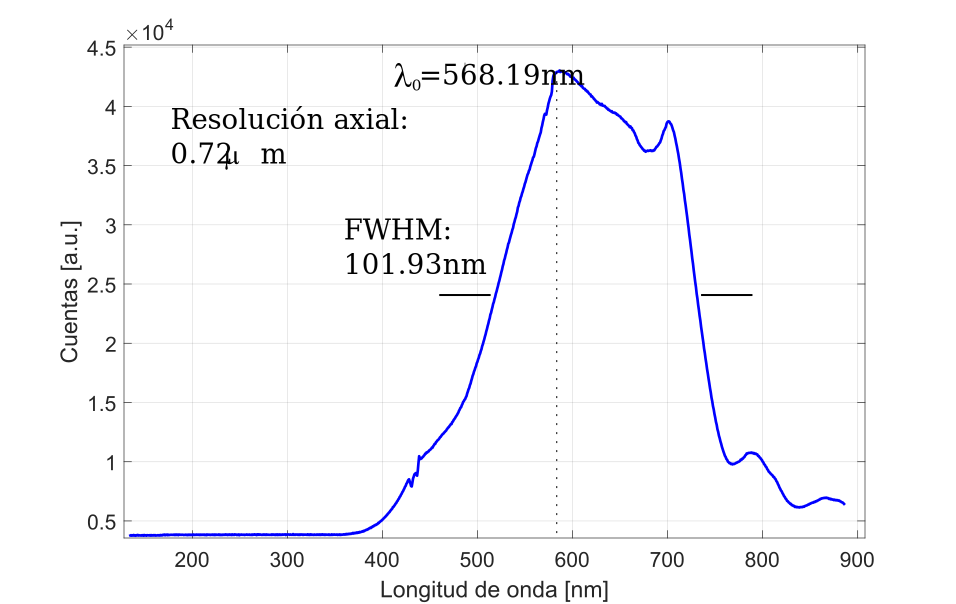
\includegraphics[width=0.49\linewidth]{img/chap2/src_spectrum}}
	\subfigure[Espectro de la fuente con filtro.]{\label{subfig:filtspectrum}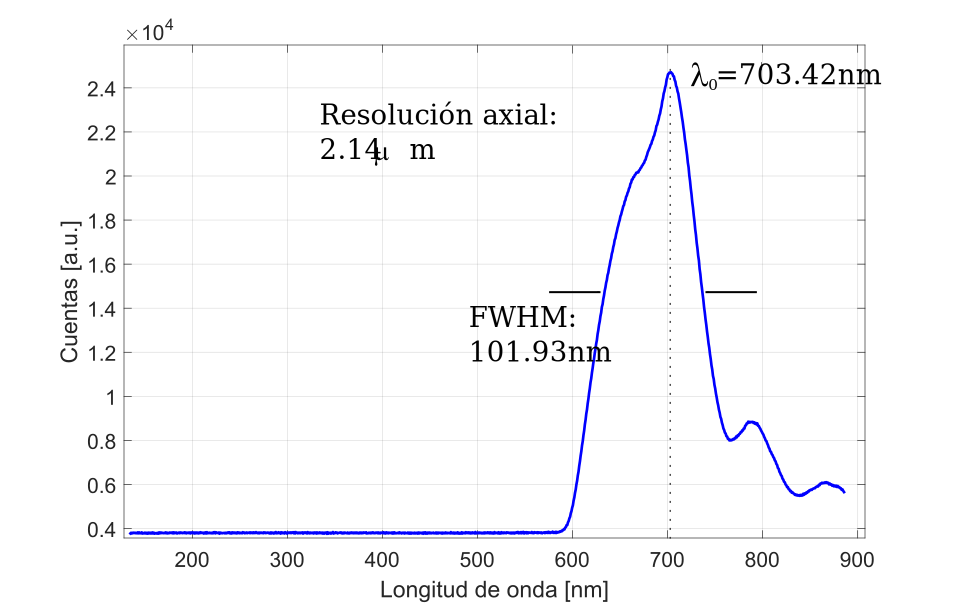
\includegraphics[width=0.49\linewidth]{img/chap2/filt_spectrum}}
	\caption[Espectro de la fuente empleada]{Espectros de la fuente halógena de tungsteno, en (a) la resolución axial es de $0.72\mu m$, mientras que en (b) corresponde a $2.14\mu m$.}
	\label{fig:spectrums}
\end{figure}

Una vez el haz ha pasado el filtro, se ubica una segunda lente (THORLABS AC254-200-A-ML) de $\phi=1"$ y distancia focal efectiva de $300mm$, con un espaciado de $5cm$ respecto a la lente, que permite enfocar el haz en la muestra, en caso de ser necesaria una mayor cantidad de luz en un área menor de la muestra. Posterior a la segunda lente, hay un cubo divisor de haz (Edmund Optics 32-702) que refleja $50\% $ de la luz incidente y transmite $50\%$. El haz transmitido, por su parte, se propaga hasta llegar a la muestra, mientras que el haz reflejado llega hasta el espejo de referencia acoplado a un desplazador piezoeléctrico (THORLABS MDT693A). El piezoeléctrico posee una resolución de $26.66nm$ por voltio y un desplazamiento máximo de $20\mu m$, éste se encuentra unido a una mesa de desplazamiento micrométrico con una resolución de $10\mu m$ y un desplazamiento máximo de $1.5cm$ para poder encontrar la región de interferencia entre los haces. Los haces reflejados vuelven al cubo divisor y pasan por una tercera lente (THORLABS LA1050) de $\phi=2"$ con distancia focal efectiva de $100mm$, que se encarga de formar imagen. El sistema formador de imagen es un $2f$, de manera que la distancia entre la lente, el espejo de referencia y la muestra es de $200mm$. Por último, en el plano imagen a $200mm$ de la última lente, se ubica una cámara CCD (Point Grey Grasshopper3 GS3-U3-91S6M-C) de $14$ bits de profundidad, resolución $3376x2704$ píxeles, tamaño de pixel $3.69\mu m$ y tasa de adquisición de datos de $9$ imágenes por segundo. Una fotografía del montaje final se presenta en la Fig.~\ref{fig:montaje}.

\begin{figure}[h!]
	\centering
	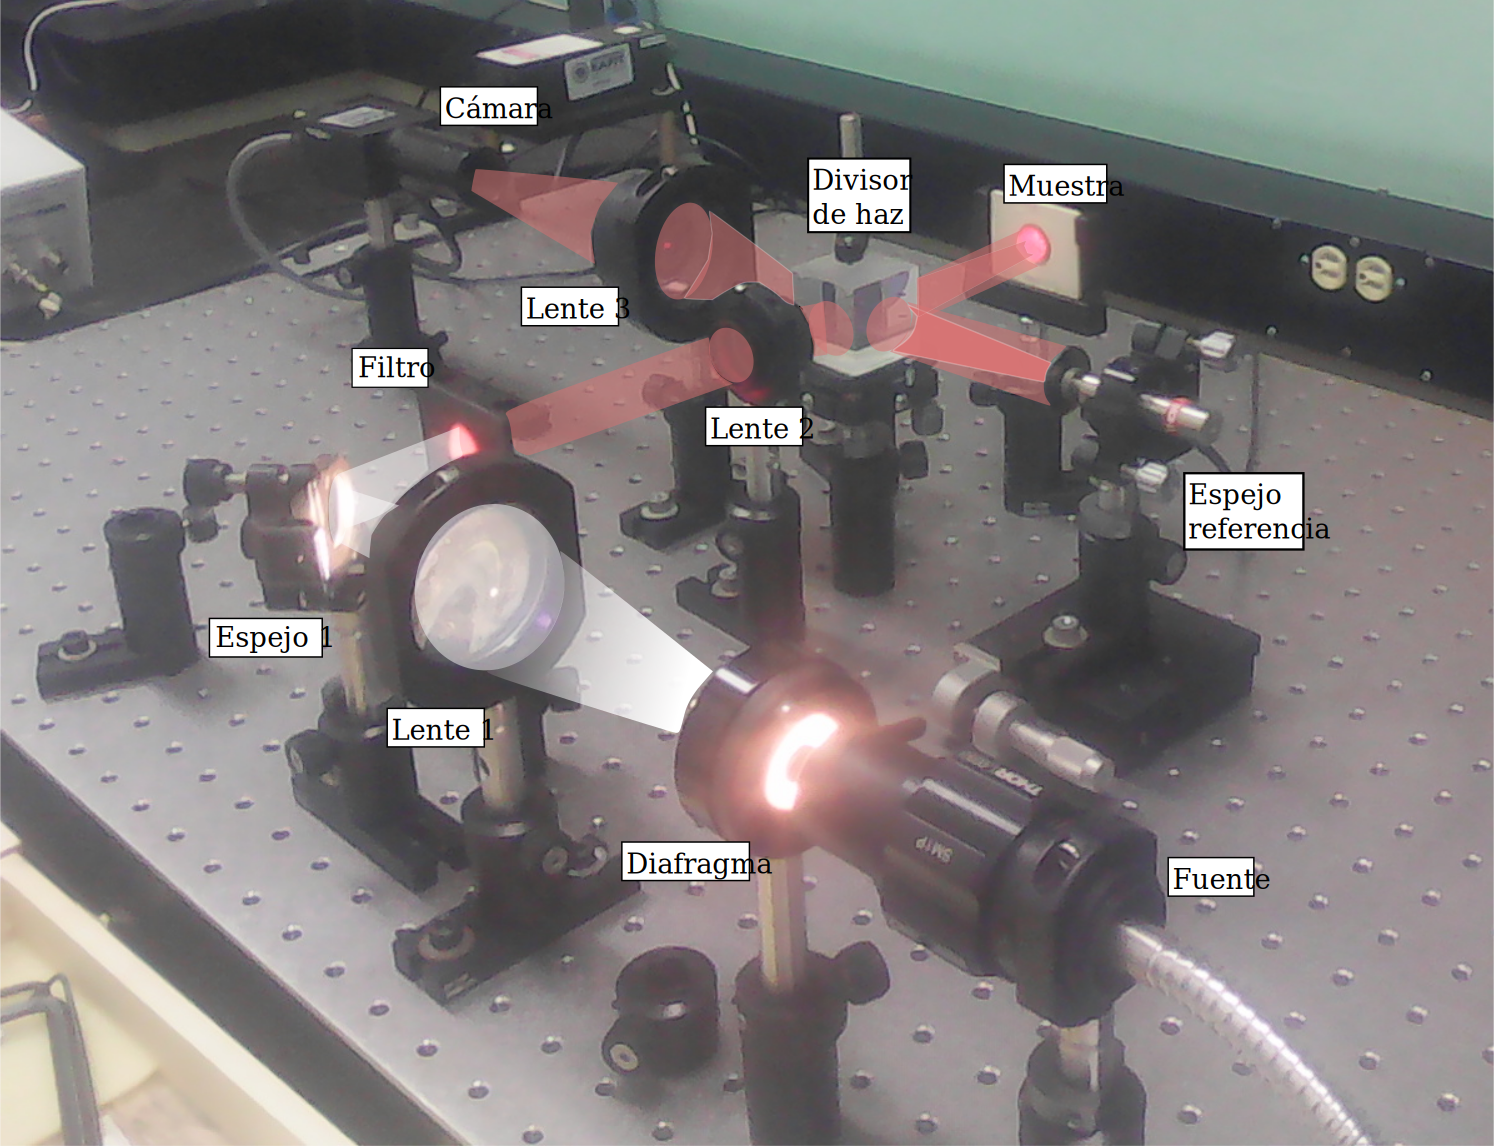
\includegraphics[width=0.8\linewidth]{img/chap2/Montaje}
	\caption[Fotografía del montaje.]{Fotografía del montaje.}
	\label{fig:montaje}
\end{figure}

\subsection{Captura de los patrones de interferencia}

La interferencia en el sistema de OCT se da unicamente cuando la diferencia de camino óptico entre el haz objeto y el haz referencia se encuentra dentro la longitud de coherencia. En el montaje implementado, ésta corresponde a $2.14\mu m$, es decir, que si la distancia recorrida por los haces que interfieren es menor que dicho rango, aparecerá un patrón de interferencia. Cuando esta distancia se obtiene, se registra el patrón que se muestra en la Fig.~\ref{subfig:patroninterferencia}. En este caso, ambos brazos poseen espejos y como el divisor de haz tiene una relación $50/50$, se espera que la interferencia sea máxima. La imagen mostrada en la Fig.~\ref{subfig:patroninterferencia} corresponde a una captura frontal del patrón, conocida en OCT como \textit{en-face}, debido a que muestra el plano $XY$ de los datos. Esta características es la base de los sistemas que emplean cámaras para capturar los patrones de interferencia, y es conocida como OCT de campo completo (FFOCT: \textit{full-field optical coherence tomography}). Como la reflectividad de la muestra se encuentra implicita en la modulación del patrón de interferencia, es necesario obtenerla mediante algoritmos similares a los de recuperación de fase, por ejemplo a partir del algoritmo de cuatro pasos \cite{Malacara1992}. En nuestro caso, se optó por emplear el algoritmo conocido como salto de fase iterativo (IPS: \textit{iterative phase shifting}) \cite{Wang2004}, este algoritmo funciona de manera similar al de cuatro pasos, pero encuentra la fase y los saltos de fase entre los interferogramas de manera iterativa, mediante un procedimiento de mínimos cuadrados. El IPS requiere al menos tres imágenes con diferentes saltos de fase, pero no requiere ninguna relación fija en los saltos de fase entre los interferogramas. Al ser un algoritmo iterativo, la precisión de la fase depende del número de iteraciones, la tolerancia del error en la función obtenida, la cantidad de imágenes que se empleen y la semilla. Empleando el IPS, con cuatro imágenes y un cambio entre iteraciones mínimo de $10^{-6}$ se obtuvo la modulación del patrón de franjas con luz blanca que se muestra en la Fig.~\ref{subfig:modulacion} en $24$ iteraciones.

\begin{figure}[ht!]
	\centering
	\subfigure[Patrón de interferencia con luz blanca.]{\label{subfig:patroninterferencia}\includegraphics[width=0.49\linewidth]{img/chap2/PatronInterferencia}}
	\subfigure[Modulación en el patrón de interferencia con luz blanca.]{\label{subfig:modulacion}\includegraphics[width=0.49\linewidth]{img/chap2/Modulacion}}
	\caption[Patrón de interferencia con luz blanca]{Patrón de interferencia obtenido a partir de luz blanca, (a) corresponde a la interferencia directa, y (b) la modulación del patrón obtenido a partir del IPS.}
	\label{fig:modulacionfranjasluzblanca}
\end{figure}

Ahora bien, si se realiza un escaneo axial tomando imágenes de las franjas de interferencia a distintas profundidades, se obtienen desplazamientos del patrón proporcionales a la profundidad en la que se encuentren. Con estos datos se reconstruye el volumen, que en este caso contiene un único reflector. Luego de capturar el volumen, si se toma el escaneo de un punto de la imagen \enface se tiene el perfil de reflectividad contra profundidad en un punto de la muestra, esto corresponde a la definición de línea A. Para el pixel central de la Fig.~\ref{subfig:patroninterferencia}, la línea A correspondiente se muestra en la Fig.~\ref{subfig:lineaa}, para esta línea la reflectividad de la muestra corresponde a su modulación, la envolvente del reflector suavizada tomando los datos obtenidos por medio del IPS se presenta en la Fig.~\ref{subfig:lineaaenvelop}. 



%La línea A muestra cómo el patrón de interferencia de la fuente depende del espectro de la fuente y de la longitud de onda central que este posee. Como se conocen los desplazamientos realizados en profundidad, en este caso, de $FALTA$, se corrobora que el ancho a la mitad del máximo corresponde a $ $, con respecto al valor teórico calculado de $2.14\mu m$, con un error del $\%$.

%Para obtener la reflectividad de la muestra, es necesario tomar el patrón de interferencia que se muestra en la Fig.~ y obtener la modulación de las franjas. 
%El objetivo de los sistemas de OCT es poder obtener la modulación en el patrón de interferencia que se produce 

\begin{figure}[ht!]
	\centering
	\subfigure[Línea A correspondiente al pixel central.]{\label{subfig:lineaa}\includegraphics[width=1\linewidth]{img/chap2/LineaAPXCenter}}
	\subfigure[Envolvente de la línea A.]{\label{subfig:lineaaenvelop}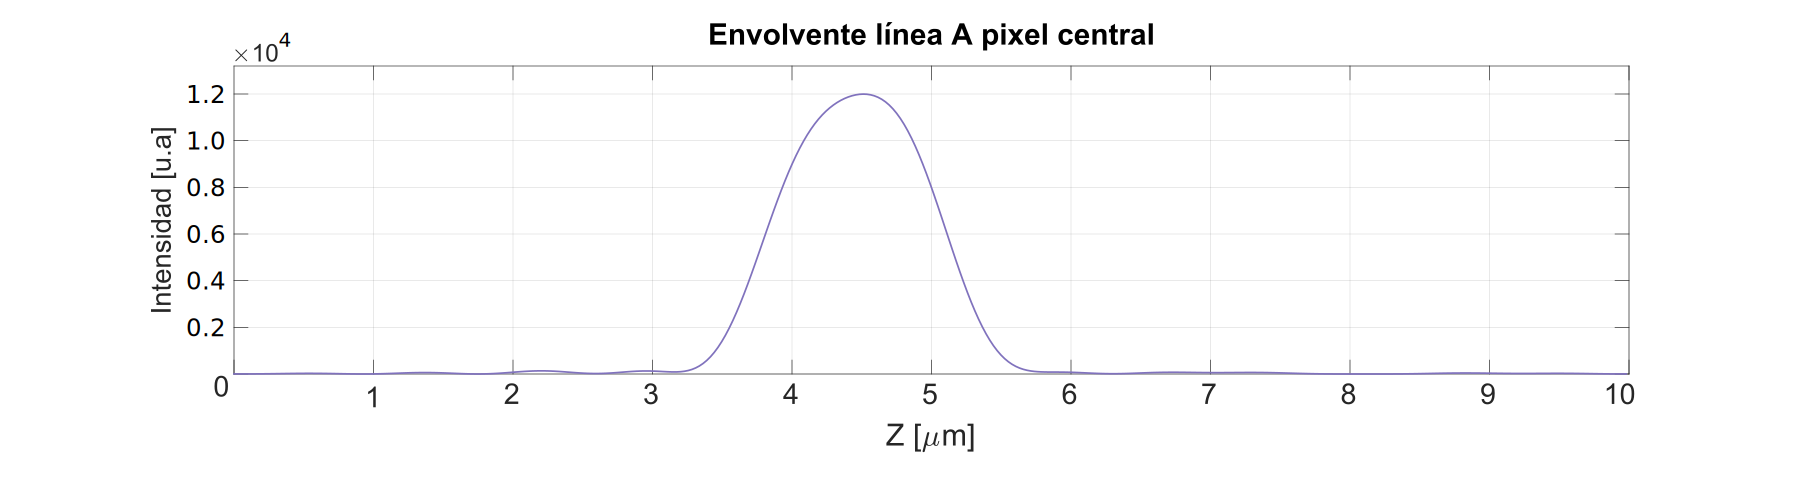
\includegraphics[width=1\linewidth]{img/chap2/LineaAPXCenterEnvelop}}
	\caption[Línea A medida experimentalmente]{Línea A correspondiente a un pixel, (a) patrón de interferencia registrado en profundidad, correspondiente a la definición de línea A, y (b) envolvente de la línea A, la altura de esta es la reflectividad de la muestra.}
	\label{fig:lineaa}
\end{figure}

%\subsubsection{Obtención de la modulación a partir del patrón de interferencia}
%
%
%
%Para obtener la modulación del patrón de franjas en un sistema de OCT, el proceso a seguir es similar al que se realiza en los algoritmos de reconstrucción de fase a partir de patrones de interferencia, por ejemplo, el algoritmo de cuatro pasos. En el algoritmo de cuatro pasos, cuatro patrones de interferencia con saltos de fase conocidos se registran $I_{1...4}$ y la fase se recupera a partir de la relación matemática
%
%\begin{equation}
%\phi = 
%\end{equation}
%
%Sin embargo, los sistemas interferométricos son altamente sensible a las vibraciones, ya que registran desplazamientos del orden de la longitud de onda. Es por ello, que para obtener la modulación, se empleó el algoritmo conocido como algoritmo de salto de fase iterativo (IPS: \textit{iterative phase shifting}). De manera similar al algoritmo de cuatro pasos, el IPS busca encontrar la fase $\phi$, con la diferencia de buscar también los saltos de fase $\delta \phi$ entre los interferogramas que se ingresan al algoritmo de manera iterativa, por lo tanto es menos sensible ante las oscilaciones del sistema. El proceso de encontrar la fase y los saltos de fase, requiere también la obtención de la modulación del patrón de interferencia, esta es la que se desea obtener en el caso de OCT.
%
%A partir de la captura de cuatro interferogramas con diferentes (y desconocidos) saltos de fase por profundidad, la modulación del patrón de interferencia mostrado en la Fig.~ puede obtenerse, esto se muestra en la Fig.~, así mismos, la modulación o envolvente de la línea A central, corresponde a la mostrada en la Fig.~.
%
Como conclusión, la obtención de la reflectividad de la muestra en cada profundidad medidas con el IPS requiere que se capturen al menos cuatro imágenes con diferentes saltos de fase \cite{Wang2004}, la ventaja fundamental de este algoritmo es que no requiere saltos de fase conocidos y por tanto es menos susceptible a vibraciones en el sistema óptico. Al ser un algoritmo iterativo, el resultado que éste brinda puede mejorarse si se incluye una cantidad mayor de interferogramas en el algoritmo, por lo tanto, cuando haya una alta absorción por parte de la muestra y un bajo contraste del patrón de interferencia, se puede incrementar la cantidad de imágenes capturadas, ya que esto ayuda a diferencia la región de la imagen con interferencia de aquellas regiones en donde se encuentra el ruido.

\subsubsection{Parámetros del montaje}

Los parámetros más importantes que determinan el desempeño del montaje y la forma en la que se midieron se relacionan a continuación:

\begin{itemize}
\item \textbf{Resolución lateral:} La resolución lateral está determinada por la capacidad para desplazarse en los ejes $x$ y $y$, en el caso de OCT de campo completo, esta resolución la indica el tamaño del pixel del detector que es $3.69\mu m$. 

\item \textbf{Resolución axial:} Determinada por la longitud de coherencia de la fuente, la resolución axial obtenida fue de $2.14\mu m$.

%\item \textbf{Profundidad de foco:} La profundidad de foco determina la región en la cual el haz enfocado no se desvía más de $\sqrt{2}w_0$, donde $w_0$ es el ancho del haz enfocado. Calculado con la Eq.~\ref{eq:depth_of_focus}, es de

%\begin{equation}
%b = \frac{4(3.16\times 10^{-6}m)}{\pi}\left( \frac{10^{-3}m}{5.08\times 10^{-3}m}\right) = 7.92\mu m
%\end{equation}

\item \textbf{Desplazamiento axial mínimo y máximo:} El paso mínimo que es posible dar en el sistema corresponde al menor desplazamiento que puede realizar el piezoeléctrico, en este caso $26.66nm$. Sin embargo, por la resolución axial, el desplazamiento se mantuvo en $1\mu m$. La distancia máxima que se puede recorrer es una combinación del desplazamiento máximo del piezoeléctrico $20\mu m$ y el desplazamiento manual que puede hacerse con el tornillo micrométrico, cuya resolución es de $10\mu m$ y un recorrido total de $1.5cm$. Para profundidades mayores a $20\mu m$, es necesario una combinación entre recorrido manual con el tornillo micrométrico y el piezoeléctrico.

\item \textbf{Sensibilidad:} La sensibilidad del sistema se midió ubicando filtros de densidad neutra de diferentes densidades en el haz objeto, instalando detrás de éste un espejo, de forma que la luz viaja dos veces por el filtro. La máxima densidad para la cual fue posible obtener interferencia fue de $1.8$, es decir, $10^{-3.6}\approx 0.25\times 10^{-3}$ veces la intensidad de entrada ó $-36dB$, considerando que la doble atenuación que sufre la luz en el filtro.


\end{itemize}

%En la Tabla~ se muestran los parámetros finales del montaje implementado

\subsection{Resultados obtenidos}
\label{sec:resultados}
\subsubsection{Topografía de la moneda}

La moneda con la cual se realizó la reconstrucción de topografía se presenta en la Fig.~\ref{fig:Moneda_Directa_img}, la zona de la imagen que se encuentra aumentada y señalada por la línea roja punteada, fue la región en la que se tomaron las imágenes. Mediante el procedimiento de recuperación de la modulación empleando ocho imágenes con el IPS a partir del patrón de franjas, se realizó un escaneo axial de la moneda con desplazamientos en la dirección $Z$ de $1\mu m$. La modulación obtenida a partir de los patrones de interferencia capturados a diferentes profundidades se muestra en la Fig.~\ref{fig:Enface_Sequence}, las regiones en donde se encuentra interferencia corresponden a las profundidades de la moneda que diferencia en altura es menor a la longitud de coherencia. 

\begin{figure}[!h]
	\centering
	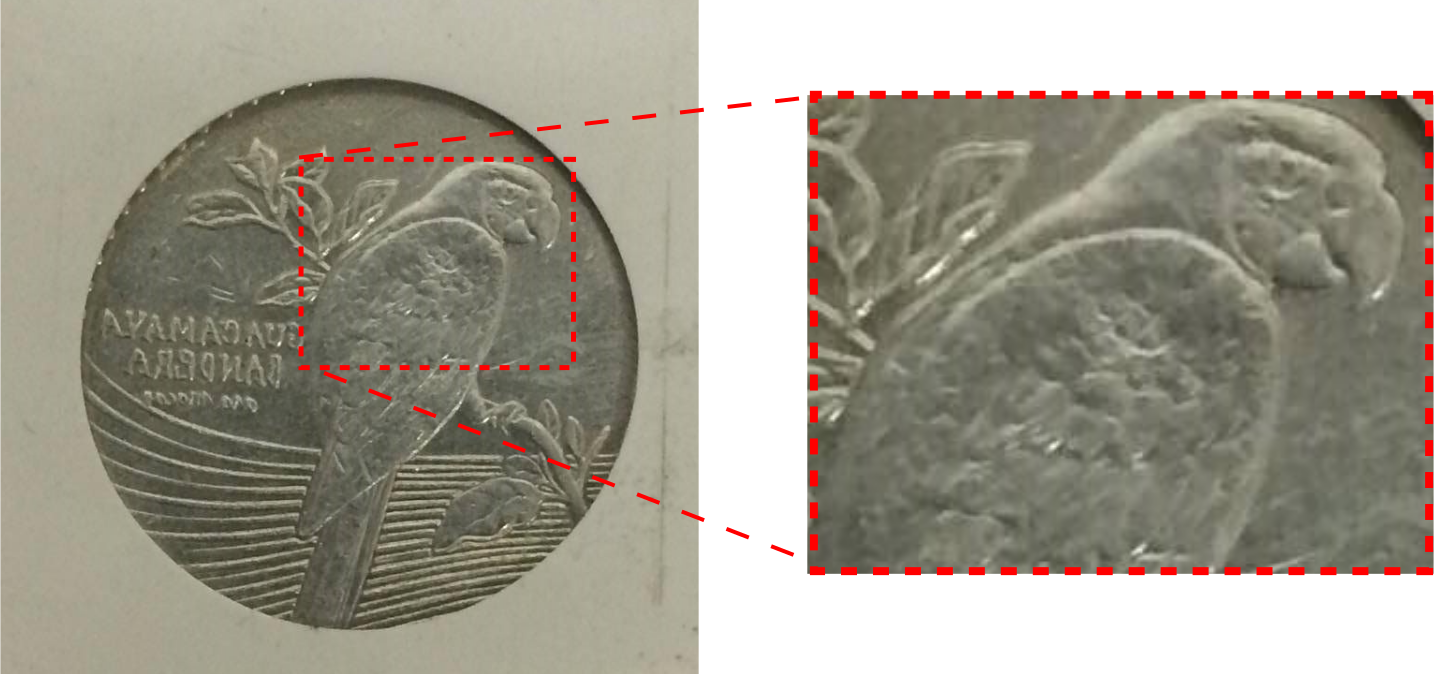
\includegraphics[width=0.6\linewidth]{img/chap2/Moneda_Directa_img}
	\caption[Moneda empleada en las mediciones.]{Moneda empleada para las mediciones con OCT, el área aumentada corresponde a la sección de la imagen capturada para la reconstrucción.}
	\label{fig:Moneda_Directa_img}
\end{figure}

Las imágenes que se presentan en la Fig.~\ref{fig:Enface_Sequence}, fueron capturadas de izquierda a derecha y de arriba hacia abajo, con una separación de $20\mu m$; en ellas se evidencia cómo la interferencia realiza un escaneo secuencial en la moneda por las diferentes profundidades del relieve que posee, comenzando por la zona inferior, en donde las características del grabado hacen que esta región del relieve se sitúe a una altura mayor, apareciendo primero en la secuencia de interferogramas. A continuación, se escanea la zona central de la moneda, hasta la parte superior, en donde se tiene la región plana y homogénea que posee la moneda. La progresión que sigue la modulación en las imágenes también indica que el haz referencia y el haz objeto no están completamente alineados, ya que la interferencia en las regiones planas de la imagen no ocurren de manera simultánea en una profundidad específica, sino que se encuentra distribuida a lo largo de diferentes profundidades.
\begin{figure}[!h]
	\centering
	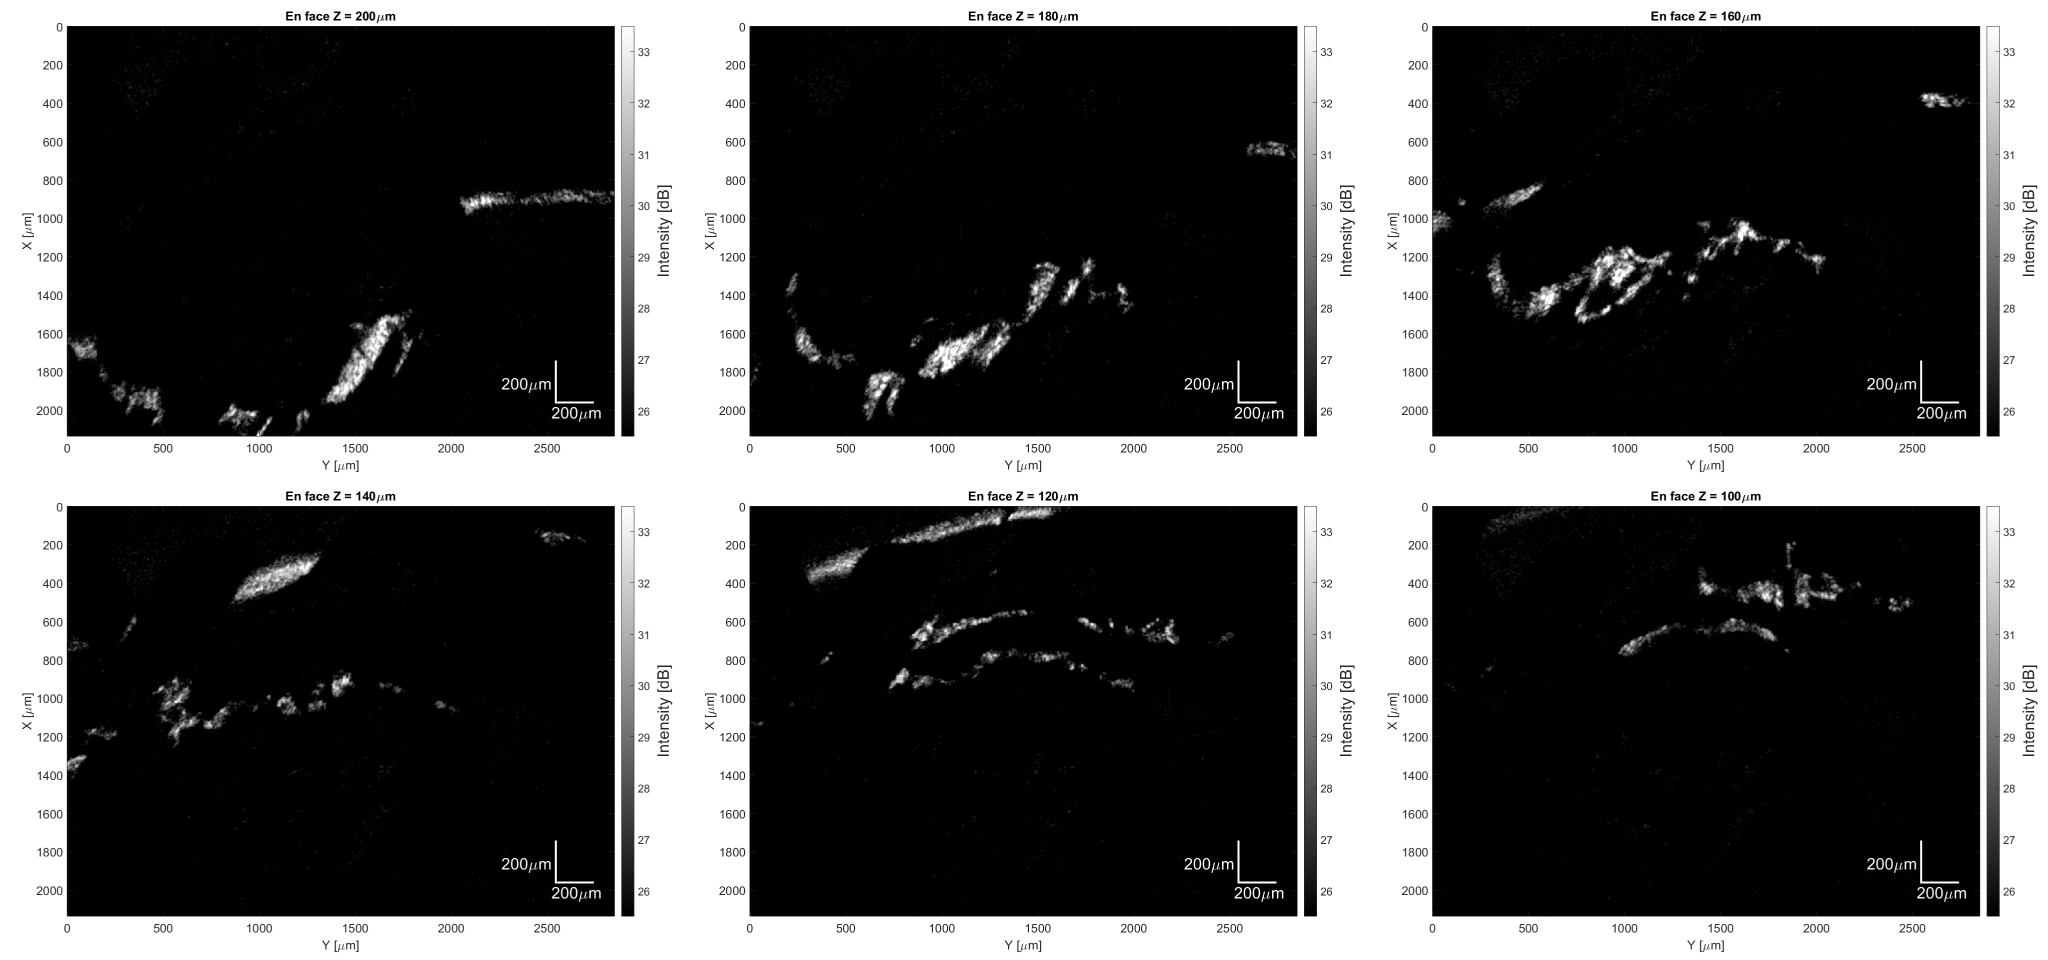
\includegraphics[width=1.0\linewidth]{img/chap2/Enface_Sequence}
	\caption[Secuencia de imágenes capturadas por la cámara.]{Secuencia de imágenes capturadas para la reconstrucción de la topografía de la moneda, la profundidad de cada imagen tiene una diferencia de $20\mu m$.}
	\label{fig:Enface_Sequence}
\end{figure}
\noindent Luego de escanear un total de $300\mu m$ en profundidad, se realizó la suma de las modulaciones obtenidas a lo largo de las diferentes posiciones axiales, ésta imagen es equivalente a la proyección bidimensional que una cámara tomaría de la moneda. El resultado de la proyección obtenida con OCT se presenta en la Fig.~\ref{subfig:monedareconstrucoct}, mientras que en la Fig.~\ref{subfig:monedaimagendirecta} se encuentra la imagen de la moneda capturada directamente por la cámara.

\begin{figure}[h!]
	\centering
	\subfigure[Imagen reconstruida a través de OCT.]{\label{subfig:monedareconstrucoct}\includegraphics[width=0.49\linewidth]{img/chap2/OCT_En_face_Projection}}
	\subfigure[Imagen directa capturada por la cámara.]{\label{subfig:monedaimagendirecta}\includegraphics[width=0.49\linewidth]{img/chap2/Direct_image_Moneda_Final}}
	\caption[Comparación de imágenes capturadas con la moneda]{Comparación de la imagen capturada directamente por la cámara con la reconstruida mediante la proyección en dirección $Z$ con OCT.}
	\label{fig:comparacionimgdirecta}
\end{figure}

Como el desplazamiento axial y el tamaño del pixel son conocidos, se pueden tomar cortes de las secciones transversales de moneda, los cuales muestran el relieve que posee a lo largo de uno de los ejes. Tomando dos secciones transversales en los ejes $ZX$ y $ZY$, ubicados en $Y = 1.06mm$ y $X = 1.71mm$ respectivamente, como se indica en líneas blancas punteadas en la Fig.~\ref{fig:OCT_Reconstruction_Moneda}, se pueden analizar algunos puntos de interés ($A-H$) en la moneda. Los puntos $A$, $B$, $C$ y $D$ se encuentran localizados a lo largo del eje $X$ y señalan en su respectivo orden: ($A$) sección plana de la moneda, ($B$) transición entre el inicio del relieve y la sección plana, ($C$) zona con alta dispersión, y ($D$) región con relieve. Los puntos $E$, $F$, $G$ y $H$ están sobre el eje $Y$, y en orden corresponden a: ($E$) primera zona plana de la moneda, ($F$) zona con alta intensidad en el relieve, ($D$) transición entre el relieve y la segunda zona plana, y ($E$) región plana. Las secciones transversales señaladas anteriormente se muestran en la Fig.~\ref{fig:monedabscan}.


\begin{figure}[!ht]
	\centering
	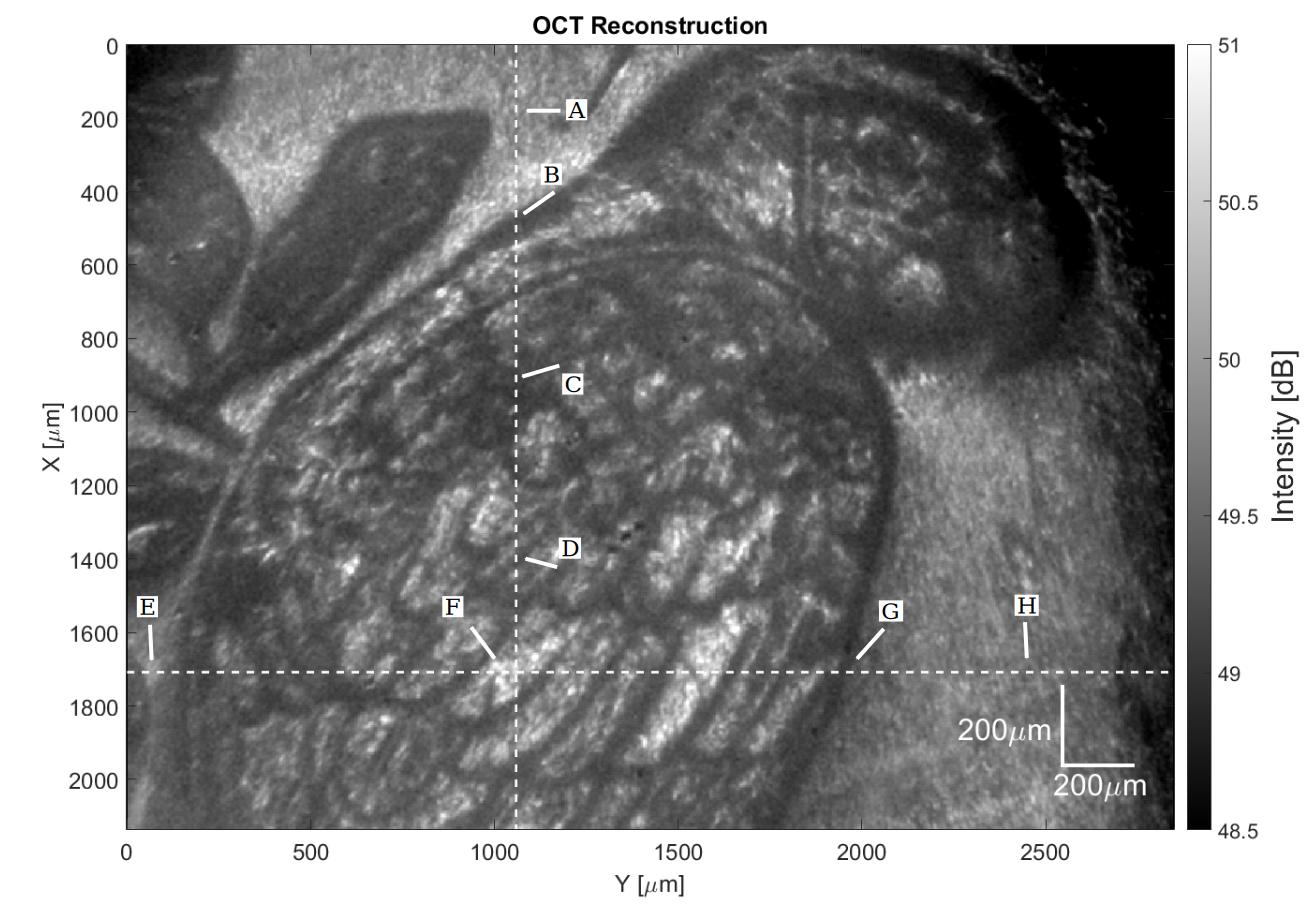
\includegraphics[width=0.7\linewidth]{img/chap2/OCT_Reconstruction_Moneda}
	\caption[Imagen de la moneda obtenida mediante la suma de todas las profundidades.]{Imagen obtenida con OCT a través de la suma de las diferentes imágenes en profundidad capturadas, esta corresponde a una captura similar a las realizadas por las cámaras. Los puntos indicados representan lugares de interés que se discuten en el texto.}
	\label{fig:OCT_Reconstruction_Moneda}
\end{figure}
La Fig.~\ref{subfig:Bscan_Moneda}, correspondiente a la sección transversal en el plano $ZX$, se le conoce como escaneo tipo B y está ubicado a una distancia $Y = 1.06mm$. En este caso, a lo largo del eje $X$ se observa unicamente la presencia de un reflector en todas las profundidades $Z$, lo que es de esperar debido a que la moneda solamente refleja luz sobre la superficie antes de absorber o reflejar la luz que llega hasta ella. Como se conoce la distancia axial escaneada y el tamaño de cada paso, se concluye que el relieve de la moneda presenta tiene una altura máxima de $\approx 50\mu m$. En la sección transversal se distinguen los puntos $A-D$ sobre el eje $X$, indicados anteriormente. El punto $A$ muestra una región plana a lo largo de $X\approx 0-500\mu m$, seguida por el punto $B$ como una zona oscura de transición a una altura mayor. $C$ aparece como una pequeña región oscura, que indica una alta dispersión de la luz en la moneda. Por último, el punto $D$ muestra una zona con fluctuaciones para $X\approx 1350-1450\mu m$. La Fig.~\ref{subfig:ZYPlane_moneda}, que es un corte en el plano $ZY$ presenta una variación en profundidad menor, pero como se mencionó, esto está relacionado con la inclinación del haz objeto con respecto al de referencia. Los puntos $E$ y $H$ muestran dos zonas donde la profundidad es constante a lo largo de $Y\approx 50-150\mu m$ y $Y\approx 2000-2800\mu m$, representando regiones planas. Alrededor del punto $F$ se encuentra una pequeña zona homogénea pero discontinua por la transición entre las diferentes alturas del relieve. El punto $G$ es la transición de la zona con relieve hasta el área plana, y es por ello que aparece como un punto opaco. Una mayor intensidad en la imagen, representa que la luz ha sido reflejada por la moneda en la dirección del detector, mientras que una baja intensidad, muestra que la moneda refleja la luz en direcciones aleatorias o la absorbe. 
\begin{figure}[h!]
	\centering
	\subfigure[Plano $ZX$ o escaneo B obtenido con la topografía de la moneda.]{\label{subfig:Bscan_Moneda}\includegraphics[width=0.97\linewidth]{img/chap2/Bscan_Moneda}}
	\subfigure[Plano $ZY$ obtenido con la topografía de la moneda.]{\label{subfig:ZYPlane_moneda}\includegraphics[width=1\linewidth]{img/chap2/ZYPlane_moneda}}
	\caption[Secciones transversales de la moneda]{Planos $ZX$ y $ZY$ reconstruidos a partir de OCT para la moneda, estos corresponden a la sección transversal. La presencia de una sola línea está asociada a que solo hay un reflector en la moneda.}
	\label{fig:monedabscan}
\end{figure}

A partir de los datos obtenidos, se realizó una reconstrucción tridimensional del volumen de datos, una secuencia de perspectivas de la topografía obtenida para la moneda a partir de este procedimiento, se encuentra en la Fig.~\ref{fig:PerspectivasTopologia}.

%En la sección transversal se distinguen estructuras regiones, tales como la zona plana de la moneda en la parte superior ($X\approx 0-200\mu m$) y las alas a lo largo del eje $X$ ($X\approx 800-2000\mu m$). Las secciones del escaneo B que aparecen oscuras, corresponden a aquellos puntos en la moneda que esparcieron más de lo reflejado, como las transiciones entre regiones a diferentes alturas (las alas, la cabe y las hojas). En la Fig.\ref{subfig:ZYPlane_moneda}, se muestra un corte de la moneda en la dirección $ZY$ en $X = 1.71mm$, de manera similar a la imagen anteriore, se observan zonas rectas ($Y \approx  2000\mu m-2500\mu m$) y con relieve en la moneda ($Y \approx  500\mu m-1700\mu m$). 



\begin{figure}
\centering
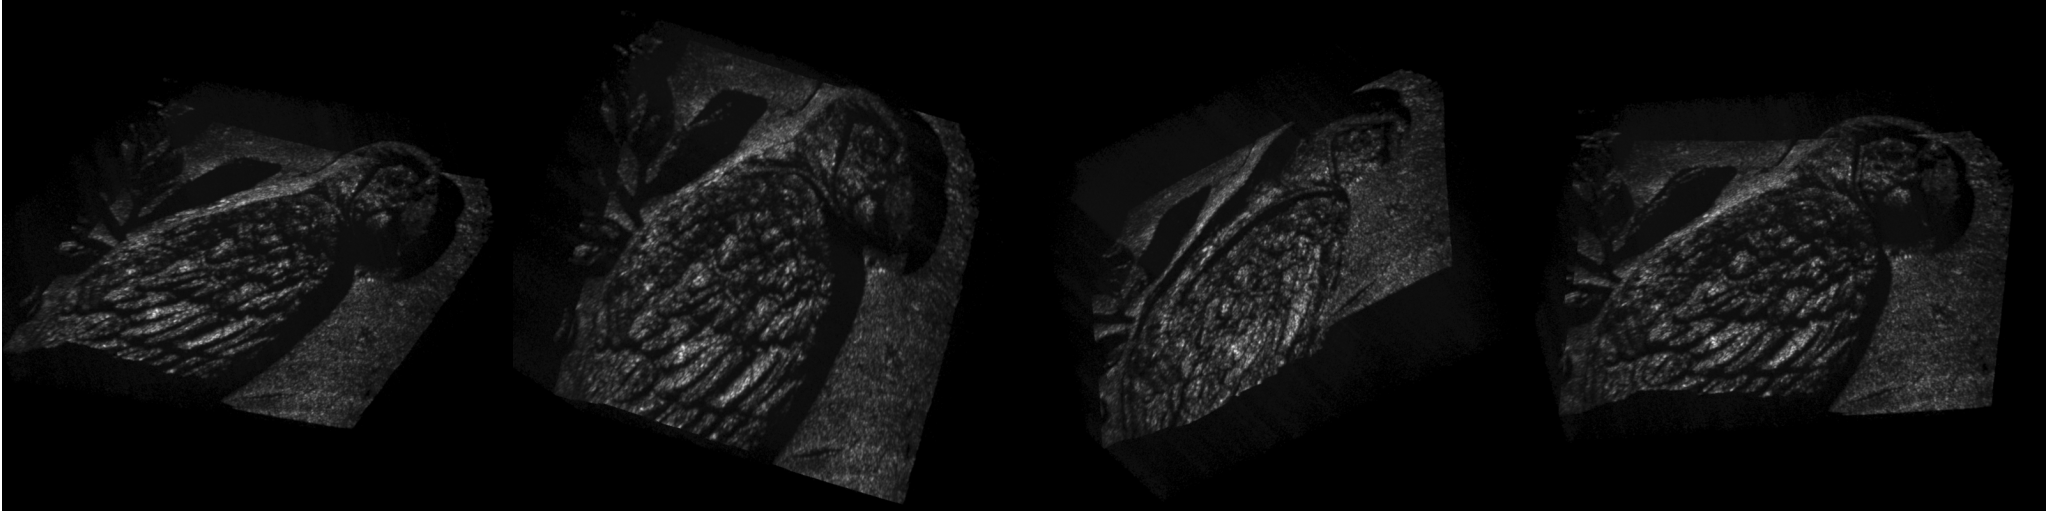
\includegraphics[width=1\linewidth]{img/chap2/PerspectivasTopologia}
\caption[Perspecivas de la topografía de la moneda.]{Secuencia de perspectivas de la topografía de la moneda reconstruidas con OCT.}
\label{fig:PerspectivasTopologia}
\end{figure}

\newpage

\subsubsection{Estructura ala de \textit{Blattodea}}


La segunda muestra que se analizó es un ala \exvivo de un insecto de la familia \emph{blattodea}, correspondiente al ala frontal conocida como \emph{tegmen}. El \emph{tegmen} en general se encuentra altamente esclerosado, es decir, endurecido por las estructuras que la conforman y la función que cumple, siendo esta última, ayudar durante el vuelo del insecto y servir como protección cuando todas las alas se encuentran plegadas. El ala empleada en las mediciones se presenta en la Fig.~\ref{fig:blattoawingzoomed}, el área que se encuentra señalada con línea punteada roja corresponde a la región de la cual se obtuvieron las imágenes. La vena más grande que se muestra en el área central de la imagen punteada y de la cual se ramifican venas más pequeñas, se conoce como \emph{radio}. El \emph{radio} cumple la función de dar el principal soporte al ala, pues contiene musculatura que ayudan a la oscilación durante el vuelo. La muestra se colocó en un portamuestras traslucido mediante un protector adhesivo.

\begin{figure}[h!]
	\centering
	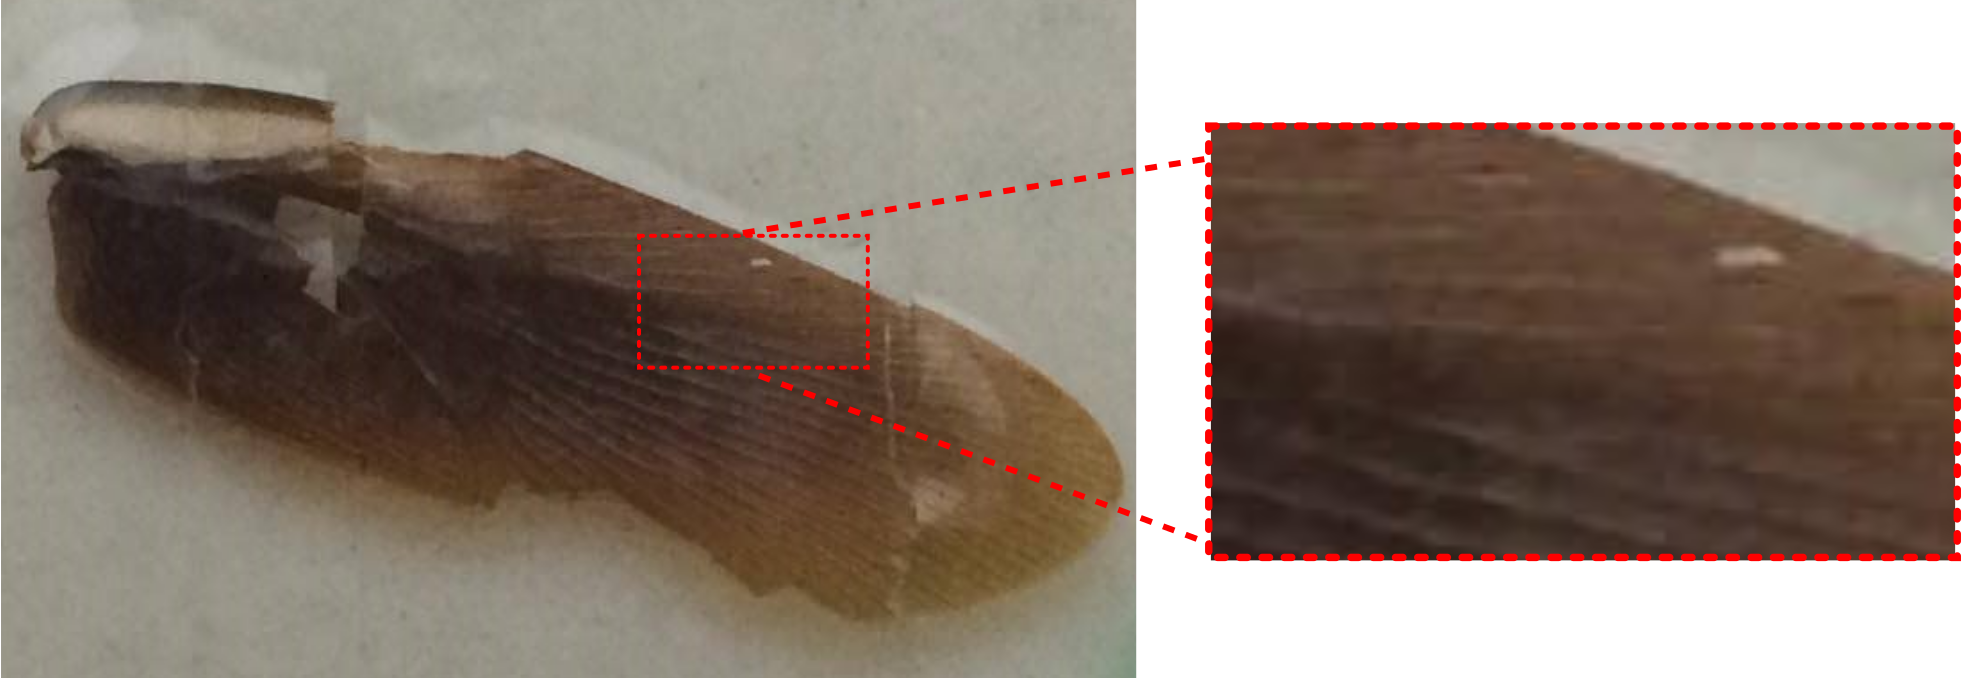
\includegraphics[width=0.7\linewidth]{img/chap2/BlattoaWingZoomed}
	\caption[Ala frontal o \emph{tegmen} de \emph{blattodea}.]{Ala frontal o \emph{tegmen}de \emph{blattodea} empleada en las mediciones. A la izquierda, fotografía de la ala, a la derecha, región a analizar.}
	\label{fig:blattoawingzoomed}
\end{figure}

De manera similar al proceso realizado para la moneda, se capturaron ocho patrones de interferencia con saltos de fase aleatorios, de forma que la modulación se recuperó a través del IPS con desplazamientos de $1\mu m$, a lo largo de una profundidad de $500\mu m$. La proyección \enface de todas las profundidades se presenta en la Fig.~\ref{fig:OCT_projection_points}, esta imagen permite distinguir algunas estructuras del ala, señaladas con flechas desde la $A$ hasta la $I$. El punto $A$ corresponde a una región en donde se observa el portamuestras, $B$ e $I$ corresponden a lugares en los cuales hay proyector adhesivo, $C$ es una vena ubicada en $X\approx 500\mu m$ aparece como una región más oscura, ya que la cantidad de luz absorbida por este tipo de estructuras se espera que sea alta; $D$ es una región de la membrana del ala y es por ello que aparece como una zona brillante, en donde la luz es altamente reflejada. $E$ aparece como una región oscura pues en esa zona la mayor parte de la luz fue absorbida por el ala, $F$ muestra un punto ubicado en el \emph{radio} del ala, y $H$ corresponde a la transición entre el ala y aire. Si se realizan dos cortes transversales a lo largo de las líneas punteadas en $X=0.6mm$ y $Y=1.72mm$, como se muestra en la Fig.\ref{fig:OCT_projection_points}, las secciones transversales con los puntos descritos anteriormente pueden analizarse desde la profundidad de la imagen, como se indican en la Fig.\ref{fig:blattodeaplanos}.
% VENA CENTRAL CORRESPONDE AL RADIO, EL BORDE DEL ALA SE CONOCE COMO COSTA, EL ALA QUE TENEMOS ES EL TEGMEN O ALA FRONTAL, EN GENERAL ESCLEROSADA (ENDURECIDA), SIRVE PARA VOLAR ASÍ COMO PROTECCIÓN PARA LAS ALAS CUANDO LAS TIENE REPLEGADAS
% IMAGEN DE COMPARACIÓN
%\begin{figure}
%	\centering
%	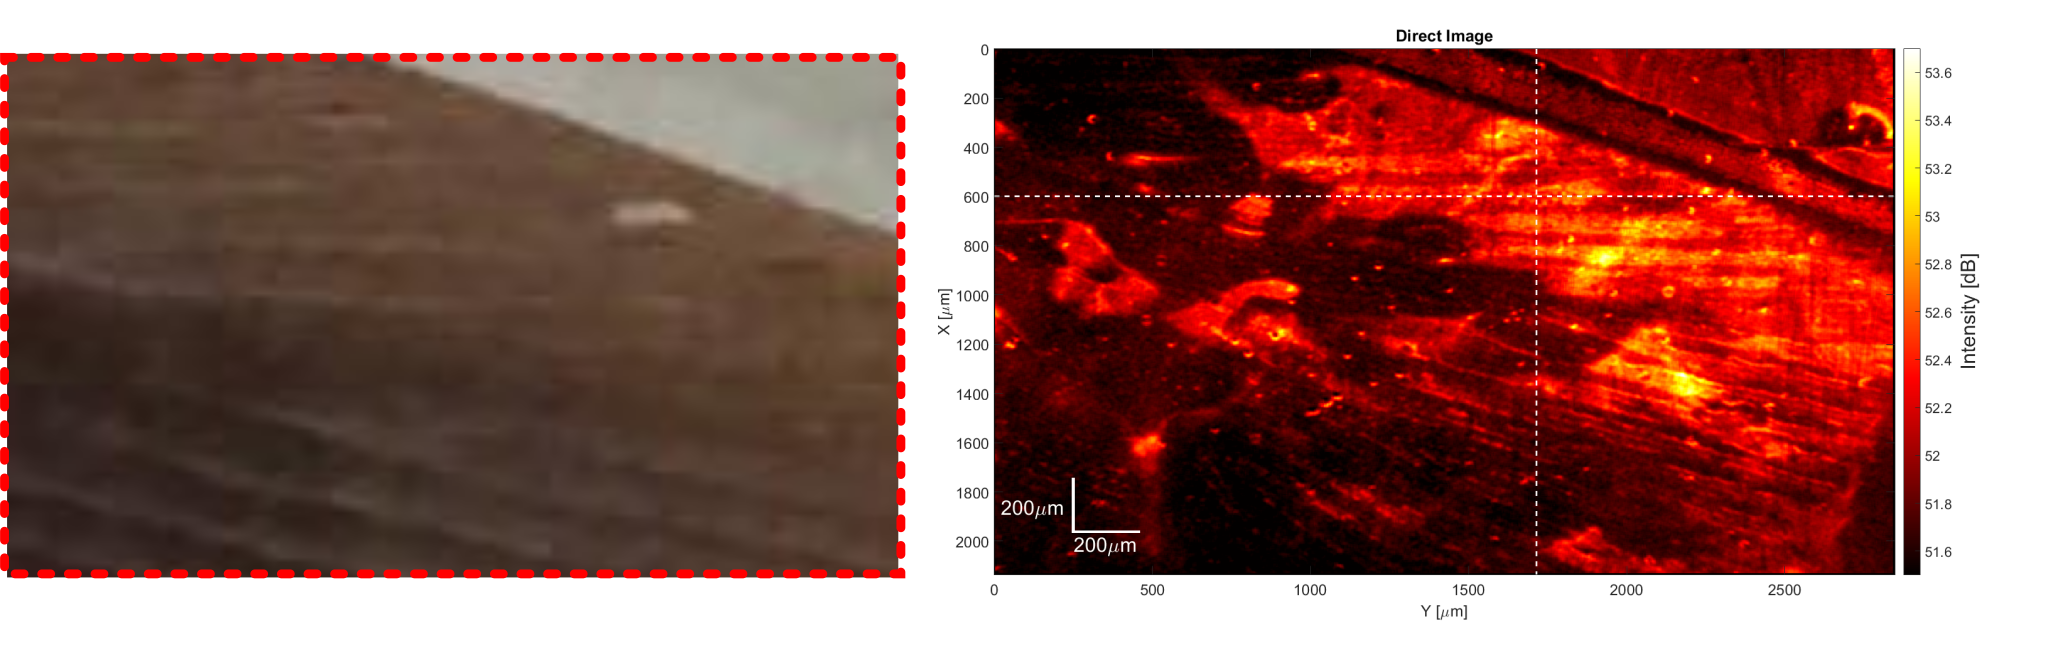
\includegraphics[width=1\linewidth]{img/chap2/WingComparisonDirect_2}
%	\caption[Imagen directa recuperada con OCT.]{Imagen directa recuperada con OCT comparada contra la región del ala analizada. Esta imagen corresponde a la superposición de todas las imágenes en profundidad obtenidas.}
%	\label{fig:wingcomparisondirect}
%\end{figure}
% UNICAMENTE INMAGEN DIRECTA
\begin{figure}[h!]
	\centering
	\includegraphics[width=0.7\linewidth]{img/chap2/OCT_projection_points}
	\caption[Imagen recuperada con OCT del ala de \textit{blattodea}.]{Imagen directa recuperada con OCT. Esta corresponde a la suma de todas las imágenes en profundidad obtenidas. Los puntos marcados son zonas de interés que se discuten en el texto. La imagen tiene un color falso de $51.5$ a $53dB$.}
	\label{fig:OCT_projection_points}
\end{figure}

%, estos dos puntos aparecen en la imagen ya que como se expicó en la Sección~\ref{sec:OCT_Esquema}, OCT registra los cambios en el índice de refracción del medio
La imagen correspondiente a la Fig.~\ref{subfig:Bscan_Wing} es el plano $ZX$ en $Y=1.72mm$, correspondiente a un escaneo tipo B para el ala, los puntos $A-E$ descritos anteriormente se han ubicado en la figura. Los puntos $PA1$ y $PA2$ refieren a la primer y segunda superficie del protector adhesivo, en general son altamente brillantes, ya que este material refleja una gran porción de la luz, y adicionalmente es la primer superficie que encuentra la luz. La región $RA$ corresponde a la ubicación del \emph{radio} del ala, y se espera que sea una región oscura porque como lo mostraba la imagen directa, ésta absorbe fuertemente la luz. Los puntos oscuros ubicados a lo largo del eje $X$ y denotados como $VA$ son venas del ala, estos puntos reflejan menos luz que la membrana dadas sus características, y por ende parecen lugares oscuros. La membrana del ala por su parte, es una estructura delgada que refleja de manera especular una alta porción de la luz, y es por ello que aparece como puntos altamente brillantes, están indicados como $ME1$ y $ME2$ para indicar la primera y la última superficie de la membrana. La línea continua indicada como $PM$ es el portamuestras sobre el que se encuentra posicionado el ala, el motivo de que no se encuentre completamente continuo se debe a que las venas atenúan fuertemente la luz, y debajo de éstas áreas es baja la reflexión. Sin embargo, nótese que por debajo del \emph{radio} ($X\approx 0.9mm$) se observa el portamuestras, es decir, aunque hayan puntos que producen sombras por la luz que atenúan, si hay una fracción de luz que penetre es posible obtener imagen de estructuras por debajo de las capas superficiales.

\begin{figure}[ht!]
	\centering
	\subfigure[Plano $ZX$ o escaneo B obtenido para el \emph{tegmen}.]{\label{subfig:Bscan_Wing}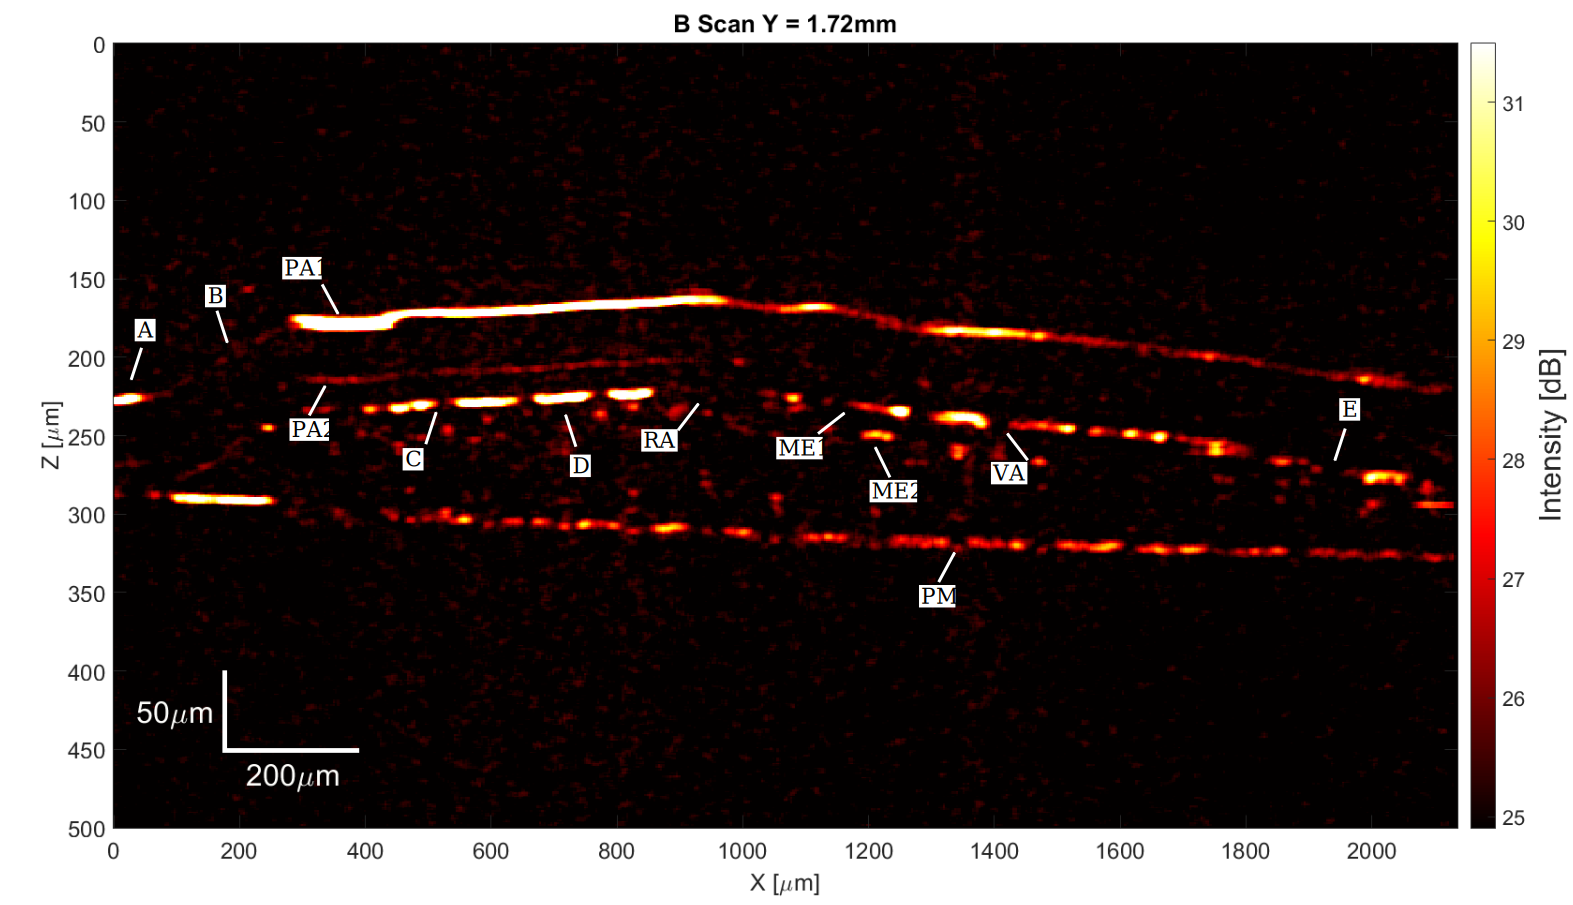
\includegraphics[width=0.8\linewidth]{img/chap2/Bscan_Wing}}
	\subfigure[Plano $ZY$ reconstruido para el \emph{tegmen}.]{\label{subfig:ZY_Wing}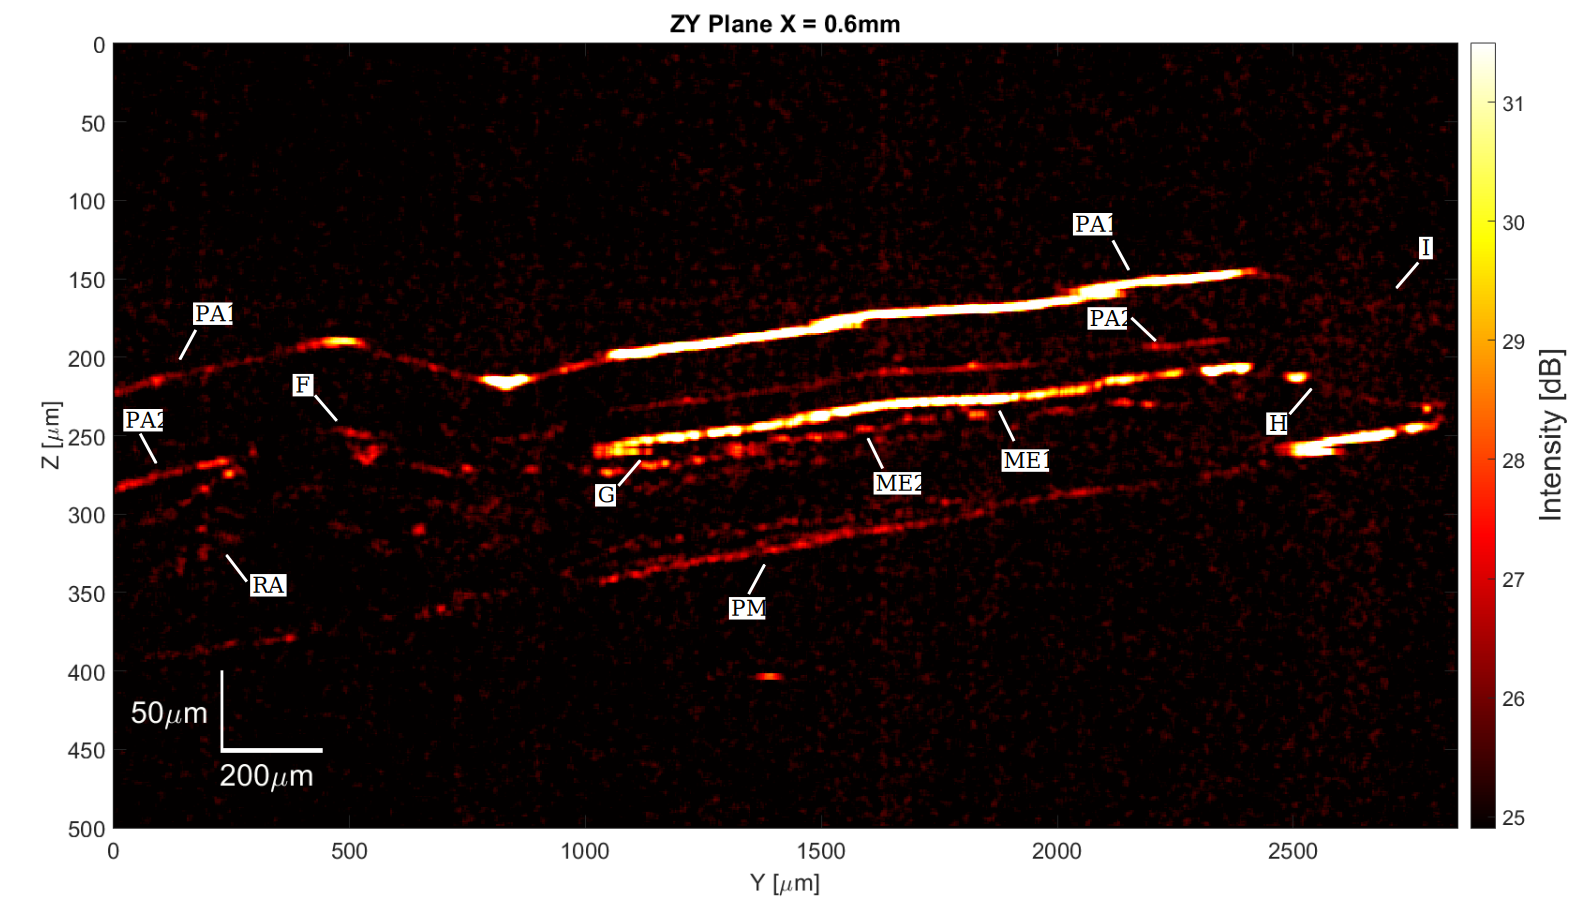
\includegraphics[width=0.8\linewidth]{img/chap2/ZY_Wing}}
	\caption[Planos de las secciones transversales del ala de \textit{blattodea}]{Planos de las secciones transversales en $ZX$ y $ZY$ reconstruidos con OCT para el \emph{tegmen}. Las imágenes tiene un color falso con un rango de $25$ a $32dB$. Los puntos indicados corresponden a: $PA1$ y $PA2$ primera y segunda superficie del protector adhesivo respectivamente, $RA$ vena correspondiente al radio de la ala, $PM$ placa portamuestras, $VA$ vena ramificada a partir del radio, $ME1$ y $ME2$ corresponden al inicio y fin de la membrana de la ala respectivamente.}
	\label{fig:blattodeaplanos}
\end{figure}

El punto $A$, indicado anteriormente, muestra una región plana de la imagen directa, si se observa este punto en la sección transversal, se aprecia que en realidad está conformado por tres capas, dos de ellas correspondiente al protector adhesivo y la última por el portamuestras. El punto $B$, conformado por las mismas capas anteriores, tiene una menor intensidad sobre el adhesivo, ya que este se encuentra inclinado con respecto al plano del detector, no obstante, el portamuestras que se encuentra alineado con el detector presenta una intensidad mucho mayor. $C$ muestra una de las diferentes venas derivadas del \emph{radio} que aparecen como puntos oscuros. $D$ está ubicado sobre una sección del ala con membrana, la que aparece como un punto brillante por la cantidad de luz que refleja. $E$ es una región oscura ya que por esa zona empieza a aparecer la región del \emph{radio}.

La Fig.~\ref{subfig:ZY_Wing} es la sección transversal del plano $ZY$ ubicado en $X=0.6mm$. El escaneo en este caso se encuentra alineado con una región de la membrana del ala, es por ello que aparece una línea que muestra claramente las dos superficies del ala $ME1$ y $ME2$. Adicionalmente, se observa como el \emph{radio} $RA$ se encuentra entre el portamuestras y el protector adhesivo, y la forma que siguen los músculos del ala. Por ejemplo en $Y\approx 1-1000\mu m$ se aprecia que el ala no se encuentra completamente alineada con el portamuestras. En este caso, no se aprecia ninguna vena por que nos encontramos en un plano paralelo que se encuentra sobre la membrana, una imagen similar a ésta se obtiene en el volumen de datos, pero mostrando la sección transversal de las venas.

Los puntos $F-I$ ubicados a lo largo del eje $X$, aparecen en este caso mostrando algunas regiones de interés. $F$ indica una región brillante sobre el \emph{radio}, bajo la cual se aprecia un pliegue del ala, y como se ve en la proyección \enface, capas más internas como el portamuestras son mucho menos visibles dada la absorción que tiene esta región. El punto $G$ está indicando la transición entre el \emph{radio} y la membrana del ala, y es por ello que aparece el cambio en el contraste. $H$ corresponde a la transición entre el ala y el portamuestras, esto se evidencia por la desaparición de la alta intensidad sobre la membrana para estar ubicada sobre el portamuestras. En el punto $I$ se observa la región donde solo el protector adhesivo y el portamuestras reflejan luz.
%El escaneo tipo B muesta varias características que con el experimento de la moneda no eran evidentes, primero que todo, en el caso del ala, se nota la presencia de múltiples reflectores a distintas profundidades para un punto específico, por ejemplo, en $X\approx 0.6mm$ se aprecia la reflexión de diferentes capas. Un ejemplo de esto, son la primer y segunda superficie del protector adhesivo $PA1$ y $PA2$ respcectivamente. 
De los resultados obtenidos, también se realizó una reconstrucción tridimensional de la estructura del ala, una secuencia de perspectivas de los resultados para el ala se presenta en la Fig.~\ref{fig:perspectivaswing}

\begin{figure}[!h]
	\centering
	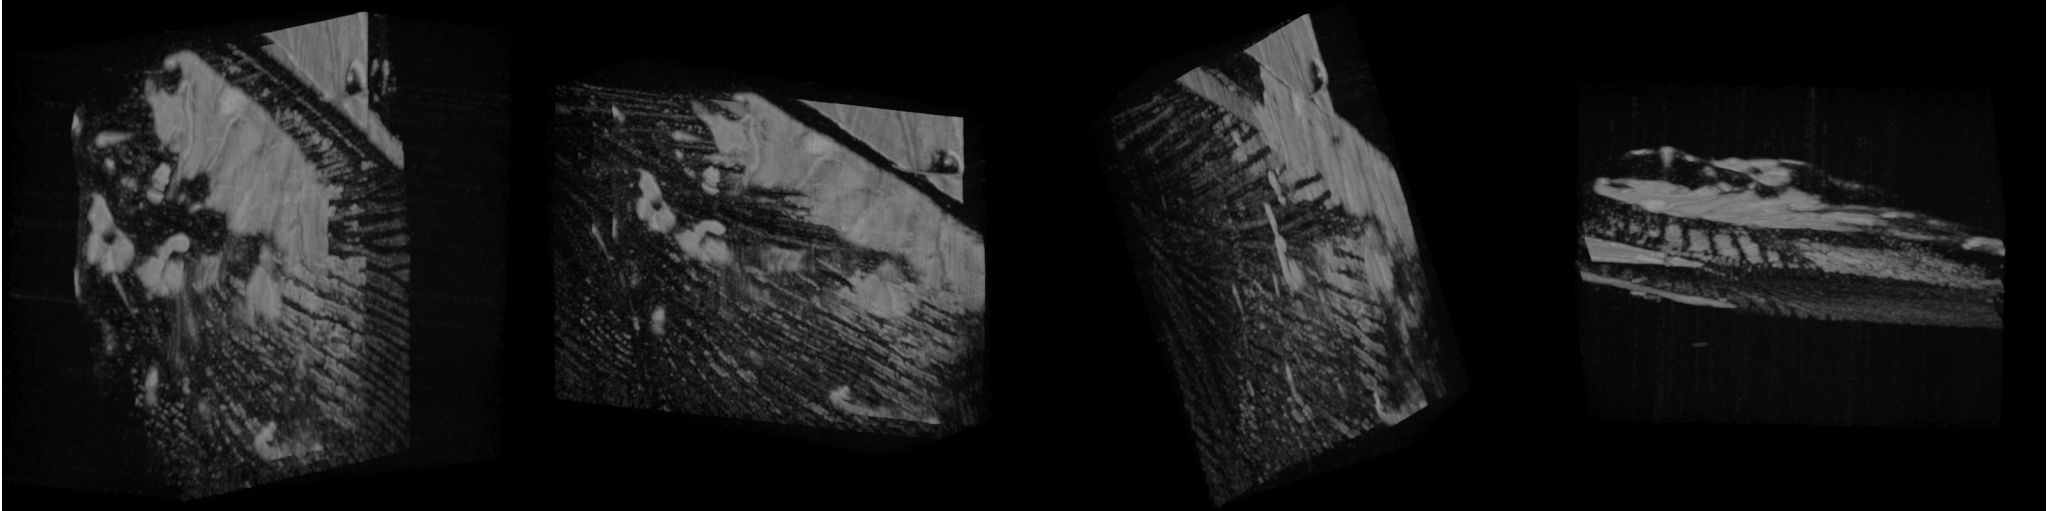
\includegraphics[width=1\linewidth]{img/chap2/Perspectivas_wing}
	\caption[Perspectivas del ala de \textit{blattodea}.]{Secuencia de perspectivas de la reconstrucción del ala.}
	\label{fig:perspectivaswing}
\end{figure}


\bibliographystyle{unsrt}
\bibliography{ref/Ref_chap_2}